\section{Expected Outputs}

The empirical outputs are designed to move from an implemented income--cost baseline to forward-looking price-risk and intervention comparisons. The latest canonical property-level modelling round already provides the first layer of this sequence: a baseline required-energy-burden engine for Westminster, built from constrained LSOA income distributions and SAP-derived required energy costs. The run labelled \texttt{20260520\_213323} covers 124,980 EPC property records across 126 LSOAs and 26 MSOAs. It preserves MSOA after-housing-cost income consistency while allowing LSOA differentiation mainly through income dispersion and lower-tail probability, rather than by claiming directly observed household incomes. A subsequent read-only sensitivity run labelled \texttt{20260526\_144256} tests alternative MSOA income anchors and the pseudo-Huber L1 lower-tail constraint; it is used here as a robustness diagnostic rather than as a replacement for the canonical property-level master.

\subsection{Implemented Baseline Outputs}

The current outputs support three baseline products. First, the model estimates LSOA lognormal income parameters, including $\mu_l$, $\sigma_l$, lower-tail probabilities below \pounds 19{,}009, and the selected MSOA-level regularisation parameter $\lambda$. In the canonical verified run, the ratio of LSOA mean income to MSOA income is tightly anchored, ranging from 0.999650 to 1.000309, while $\sigma_l$ ranges from 0.4192 to 1.4000. Only 3 of 126 LSOAs sit at the new upper bound, compared with 31 of 126 under the previous bound of 0.9. This indicates that within-MSOA differentiation is being carried primarily by dispersion and tail probability.

Second, the model produces property-level SAP-derived required energy cost and the probability that required energy burden exceeds a 10 percent threshold. This output should be interpreted as baseline required-energy affordability exposure, not as a complete household fuel price risk measure. It provides the denominator and cost foundation for later shock scenarios, while avoiding dependence on actual expenditure that may be suppressed by underheating or self-rationing.

The 2026-05-28 baseline extract turns this layer into a fixed shock-engine input. The extract reports a median SAP-inverse required energy cost of approximately \pounds 1,045 per year, a median EPC component cost of approximately \pounds 651 per year, and a median deterministic baseline required energy burden of 0.0239 under the MSOA point-income denominator. Figure~\ref{fig:baseline-burden-distribution} shows the corresponding deterministic burden distribution. Only 0.6 percent of properties exceed the 10 percent burden threshold under this point-income measure, which is why the deterministic ratio should not be treated as the whole exposure story.

\begin{figure}[H]
\centering
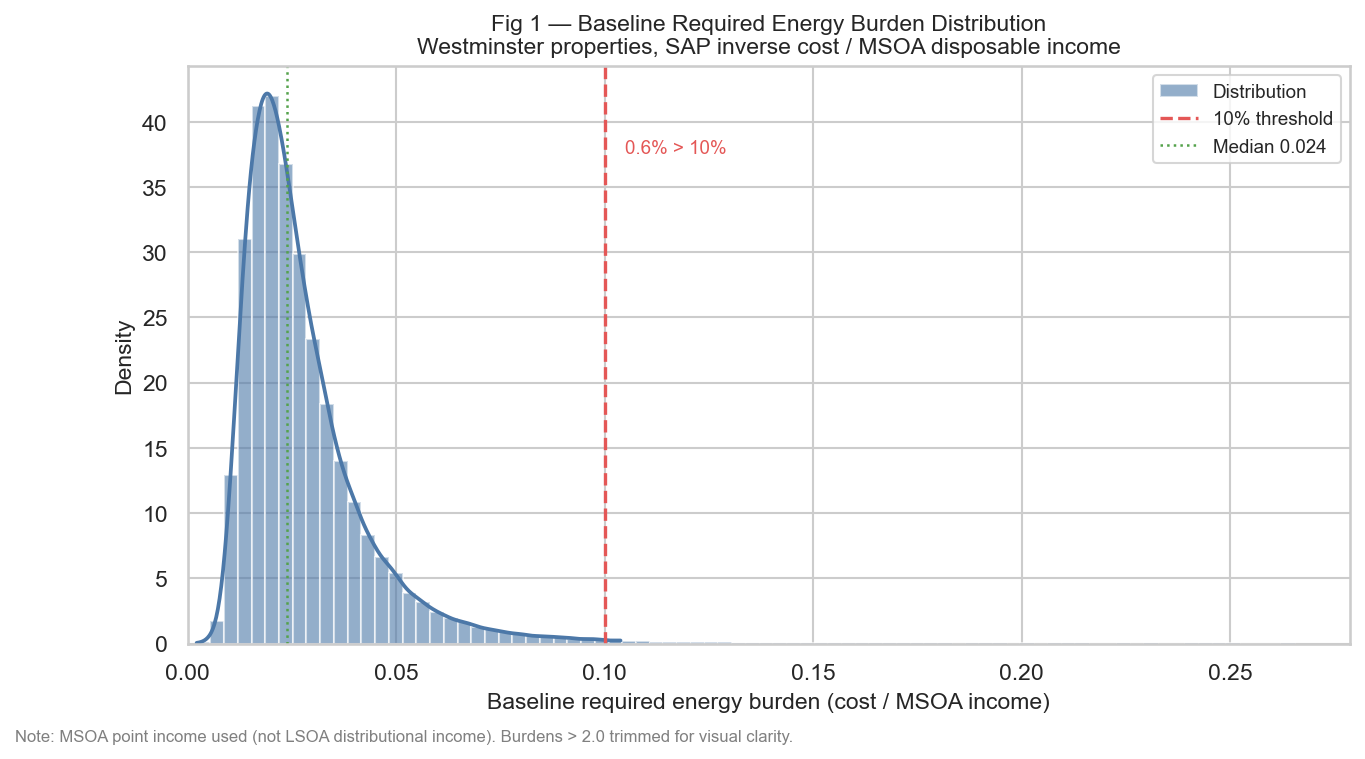
\includegraphics[width=\linewidth]{paper/figures/baseline_required_energy_burden_distribution.png}
\caption{Baseline required energy burden distribution for Westminster properties, using SAP-inverse required energy cost divided by MSOA disposable income. The figure shows the current-price point-income burden metric; it is a baseline affordability measure, not a future fuel-price-shock result.}
\label{fig:baseline-burden-distribution}
\end{figure}

Figure~\ref{fig:burden-prob-distribution} reports the distributional counterpart: the probability that required energy burden exceeds 10 percent when local LSOA income distributions are used. Its median is 0.0525, and the top-decile threshold used for the HR\_TOP10 burden-probability group is 0.311. The contrast between Figures~\ref{fig:baseline-burden-distribution} and \ref{fig:burden-prob-distribution} is substantively important. It shows why Westminster exposure cannot be inferred from a single area-income point estimate: the point burden is usually low, while the income-tail probability has a much wider distribution.

\begin{figure}[H]
\centering
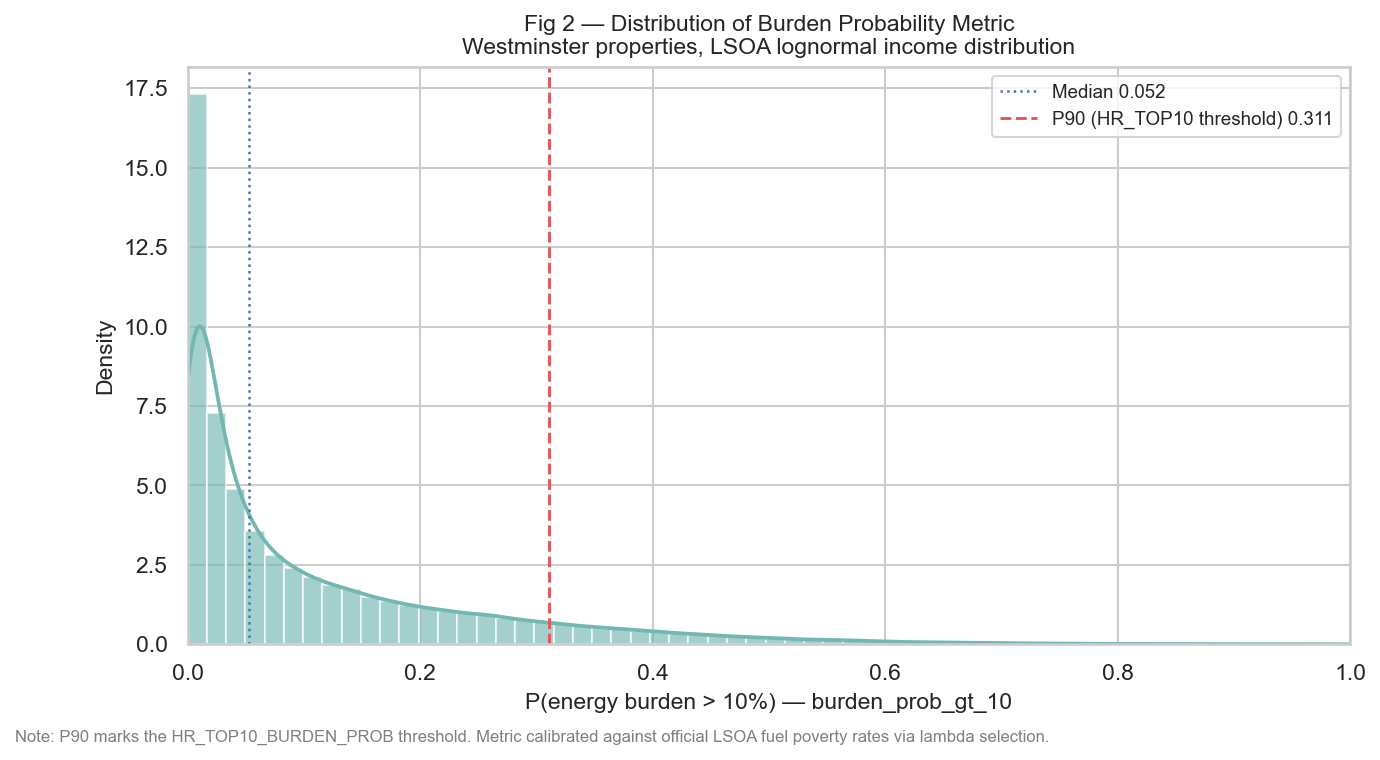
\includegraphics[width=\linewidth]{paper/figures/baseline_burden_probability_distribution.png}
\caption{Distribution of the baseline burden-probability metric, \texttt{burden\_prob\_gt\_10}. The metric uses constrained LSOA lognormal income distributions to estimate the probability that required energy burden exceeds 10 percent. It identifies current income-tail exposure and does not yet include price-shock scenarios.}
\label{fig:burden-prob-distribution}
\end{figure}

The extract also clarifies the housing and fuel composition of the current high-burden tail. Figure~\ref{fig:baseline-high-burden-property-type} shows that flats dominate Westminster's overall stock, but houses and maisonettes are overrepresented in high-burden groups relative to their stock share. Figure~\ref{fig:baseline-high-burden-main-fuel} shows that gas dominates all groups because it dominates the stock, while electricity's share rises slightly in the HR groups. These figures support a layered interpretation: current burden exposure is produced by stock composition, property type, required demand, income distribution, and fuel exposure together, not by one variable alone.

\begin{figure}[H]
\centering
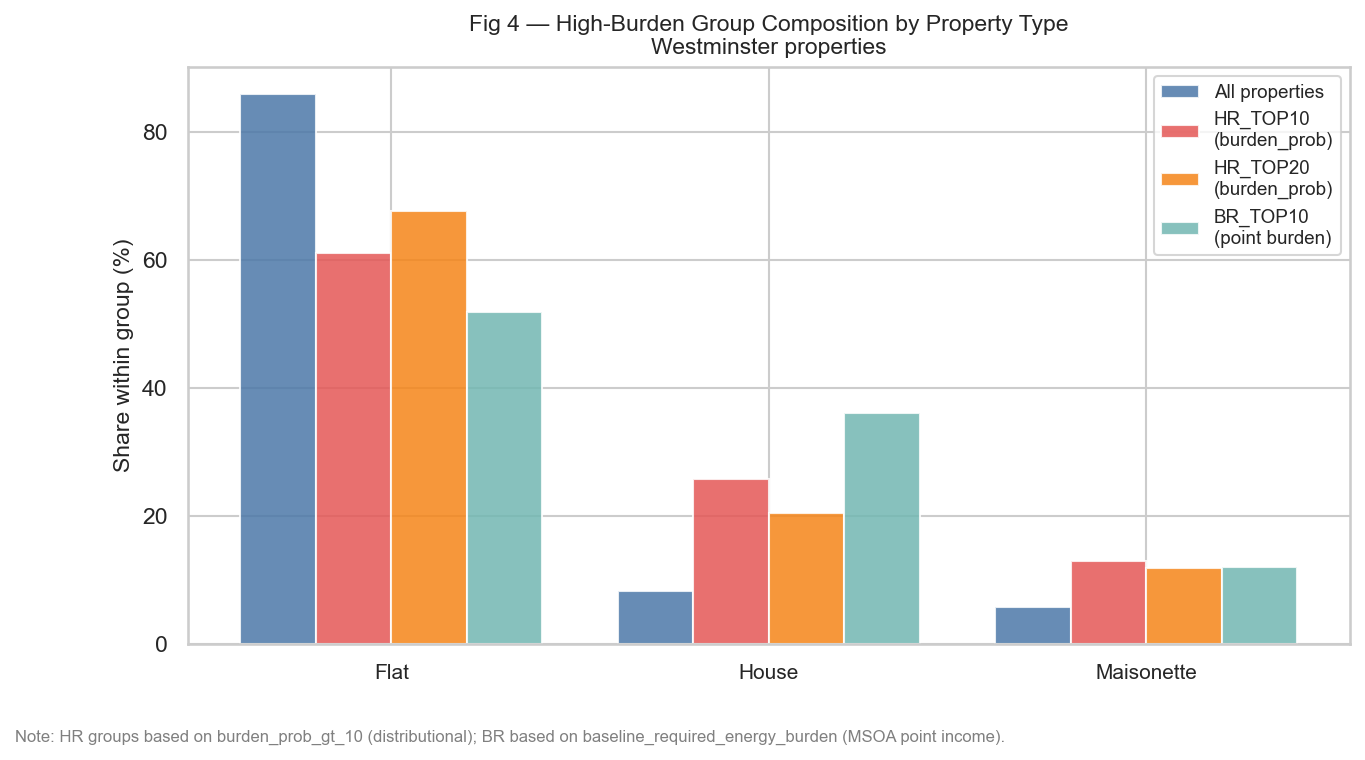
\includegraphics[width=\linewidth]{paper/figures/baseline_high_burden_by_property_type.png}
\caption{Composition of baseline high-burden groups by property type. HR groups are based on \texttt{burden\_prob\_gt\_10}; BR groups are based on deterministic baseline required energy burden using MSOA point income.}
\label{fig:baseline-high-burden-property-type}
\end{figure}

\begin{figure}[H]
\centering
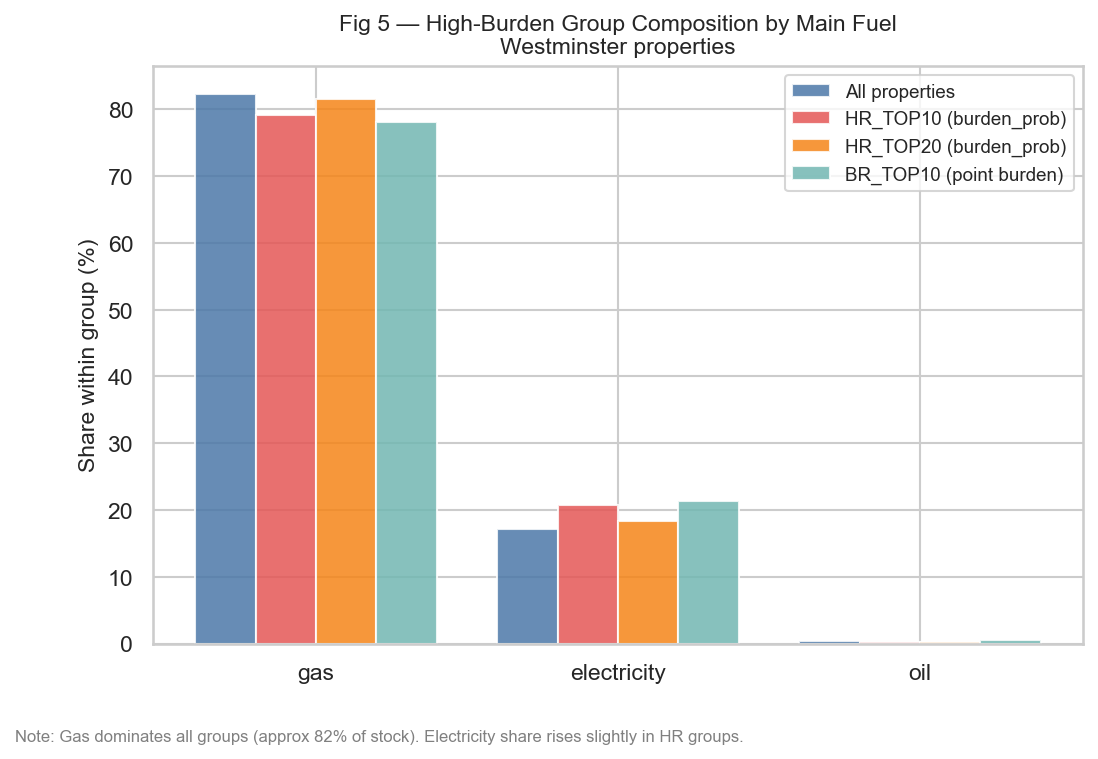
\includegraphics[width=0.86\linewidth]{paper/figures/baseline_high_burden_by_main_fuel.png}
\caption{Composition of baseline high-burden groups by main fuel. The figure shows gas dominance in the stock and a modest overrepresentation of electricity in the HR groups; it motivates fuel-specific price-shock modelling rather than claims about completed fuel price risk.}
\label{fig:baseline-high-burden-main-fuel}
\end{figure}

Third, the baseline module generates a modelled LSOA fuel-poverty comparison used for calibration diagnostics. The latest sensitivity run has a mean modelled-minus-official LSOA fuel-poverty-rate error of -0.0174 and a worst absolute error of 0.133 under the central income-anchor scenario. Weighted MSOA-level RMSE is similar across the central, upper-confidence-limit, and lower-confidence-limit scenarios, with means of 0.04944, 0.05022, and 0.04821 respectively. This residual gap is substantively useful rather than merely technical: it shows that income-tail matching alone does not reproduce official fuel-poverty geography, reinforcing the paper's distinction between income deprivation, required energy burden, dwelling fabric, heating systems, tenure, and future price risk.

Figures~\ref{fig:lsoa-income-pdf-scenarios-1}--\ref{fig:lsoa-income-pdf-scenarios-3} report the promoted LSOA income PDF scenario panels from the May 2026 read-only sensitivity run. They should be read as sensitivity diagnostics for the synthetic income layer. The solid, dashed, and dotted curves compare central, upper-confidence-limit, and lower-confidence-limit MSOA income anchors while holding the lower-tail constraint and required-energy-cost logic fixed. The red vertical marker is the \pounds 19{,}009 income-tail threshold used in the current module. These figures therefore support the baseline burden model by showing how local lower-tail assumptions vary across LSOAs and MSOAs; they do not yet measure future household fuel price risk.

\begin{figure}[H]
\centering
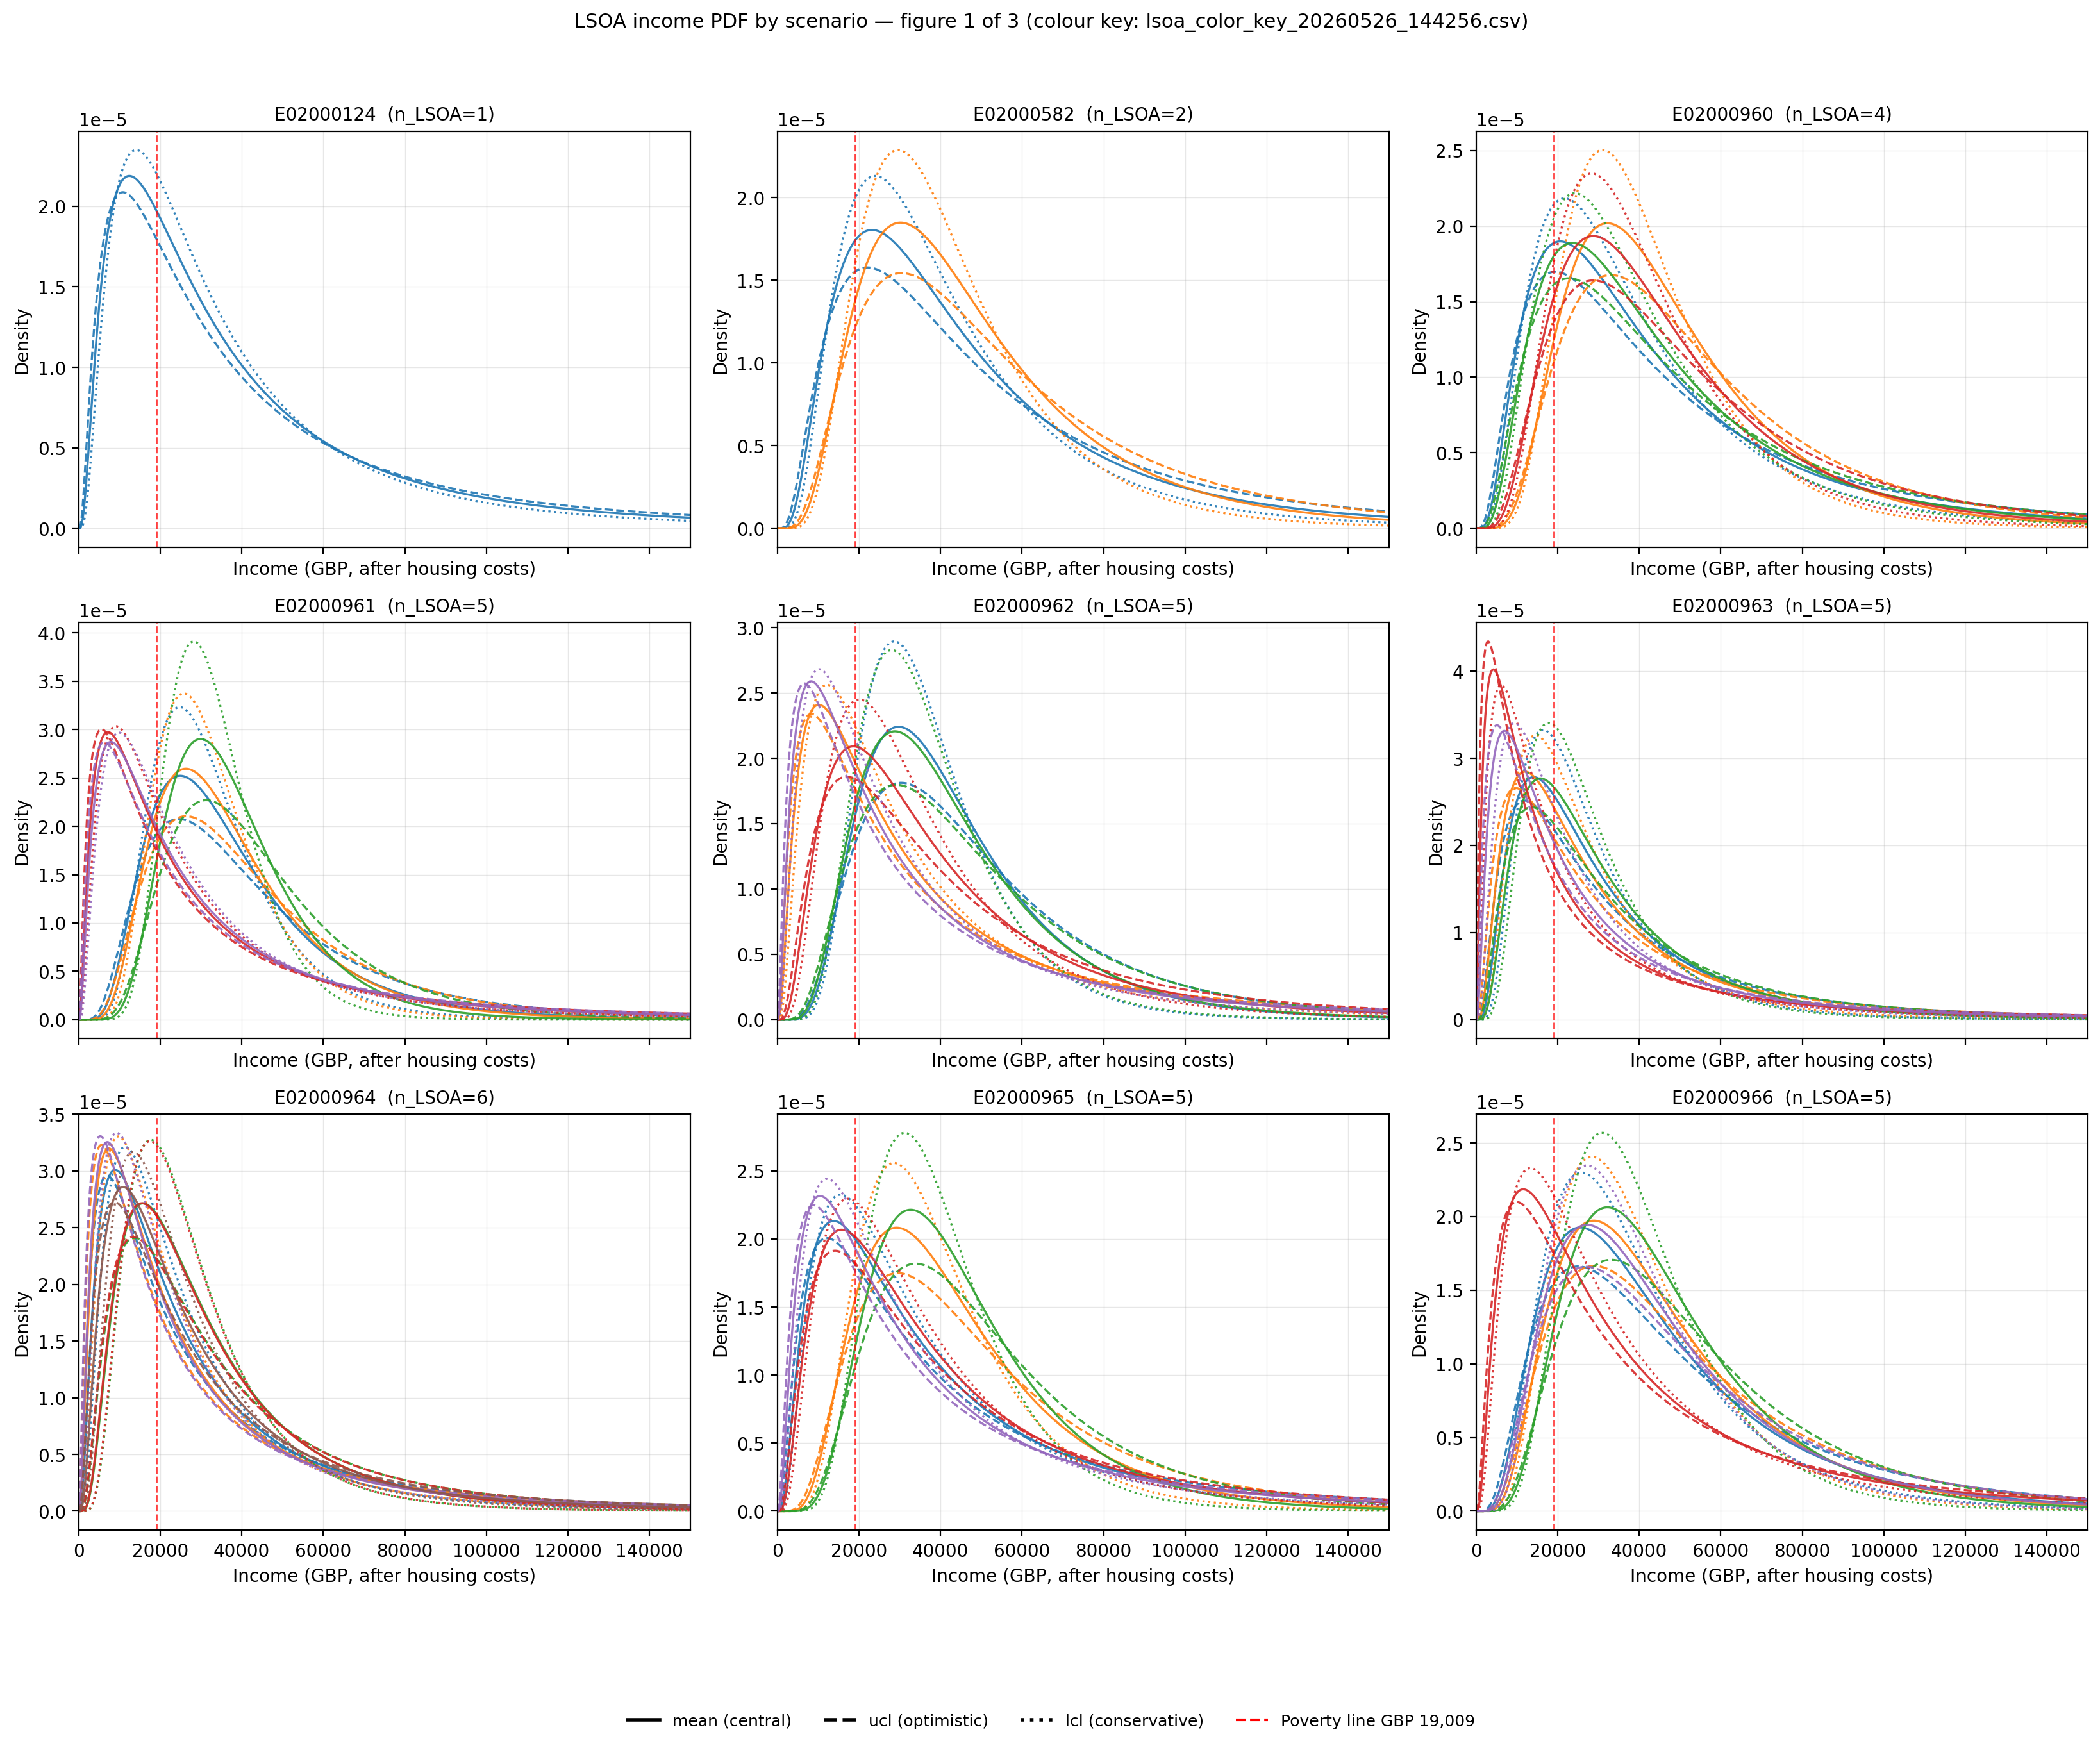
\includegraphics[width=\linewidth]{paper/figures/baseline_income_pdf_scenarios_1.png}
\caption{LSOA income PDF scenario sensitivity, panel set 1 of 3. The curves compare central, upper-confidence-limit, and lower-confidence-limit MSOA after-housing-cost income anchors for constrained synthetic LSOA income distributions; the red line marks the \pounds 19{,}009 lower-tail threshold.}
\label{fig:lsoa-income-pdf-scenarios-1}
\end{figure}

\begin{figure}[H]
\centering
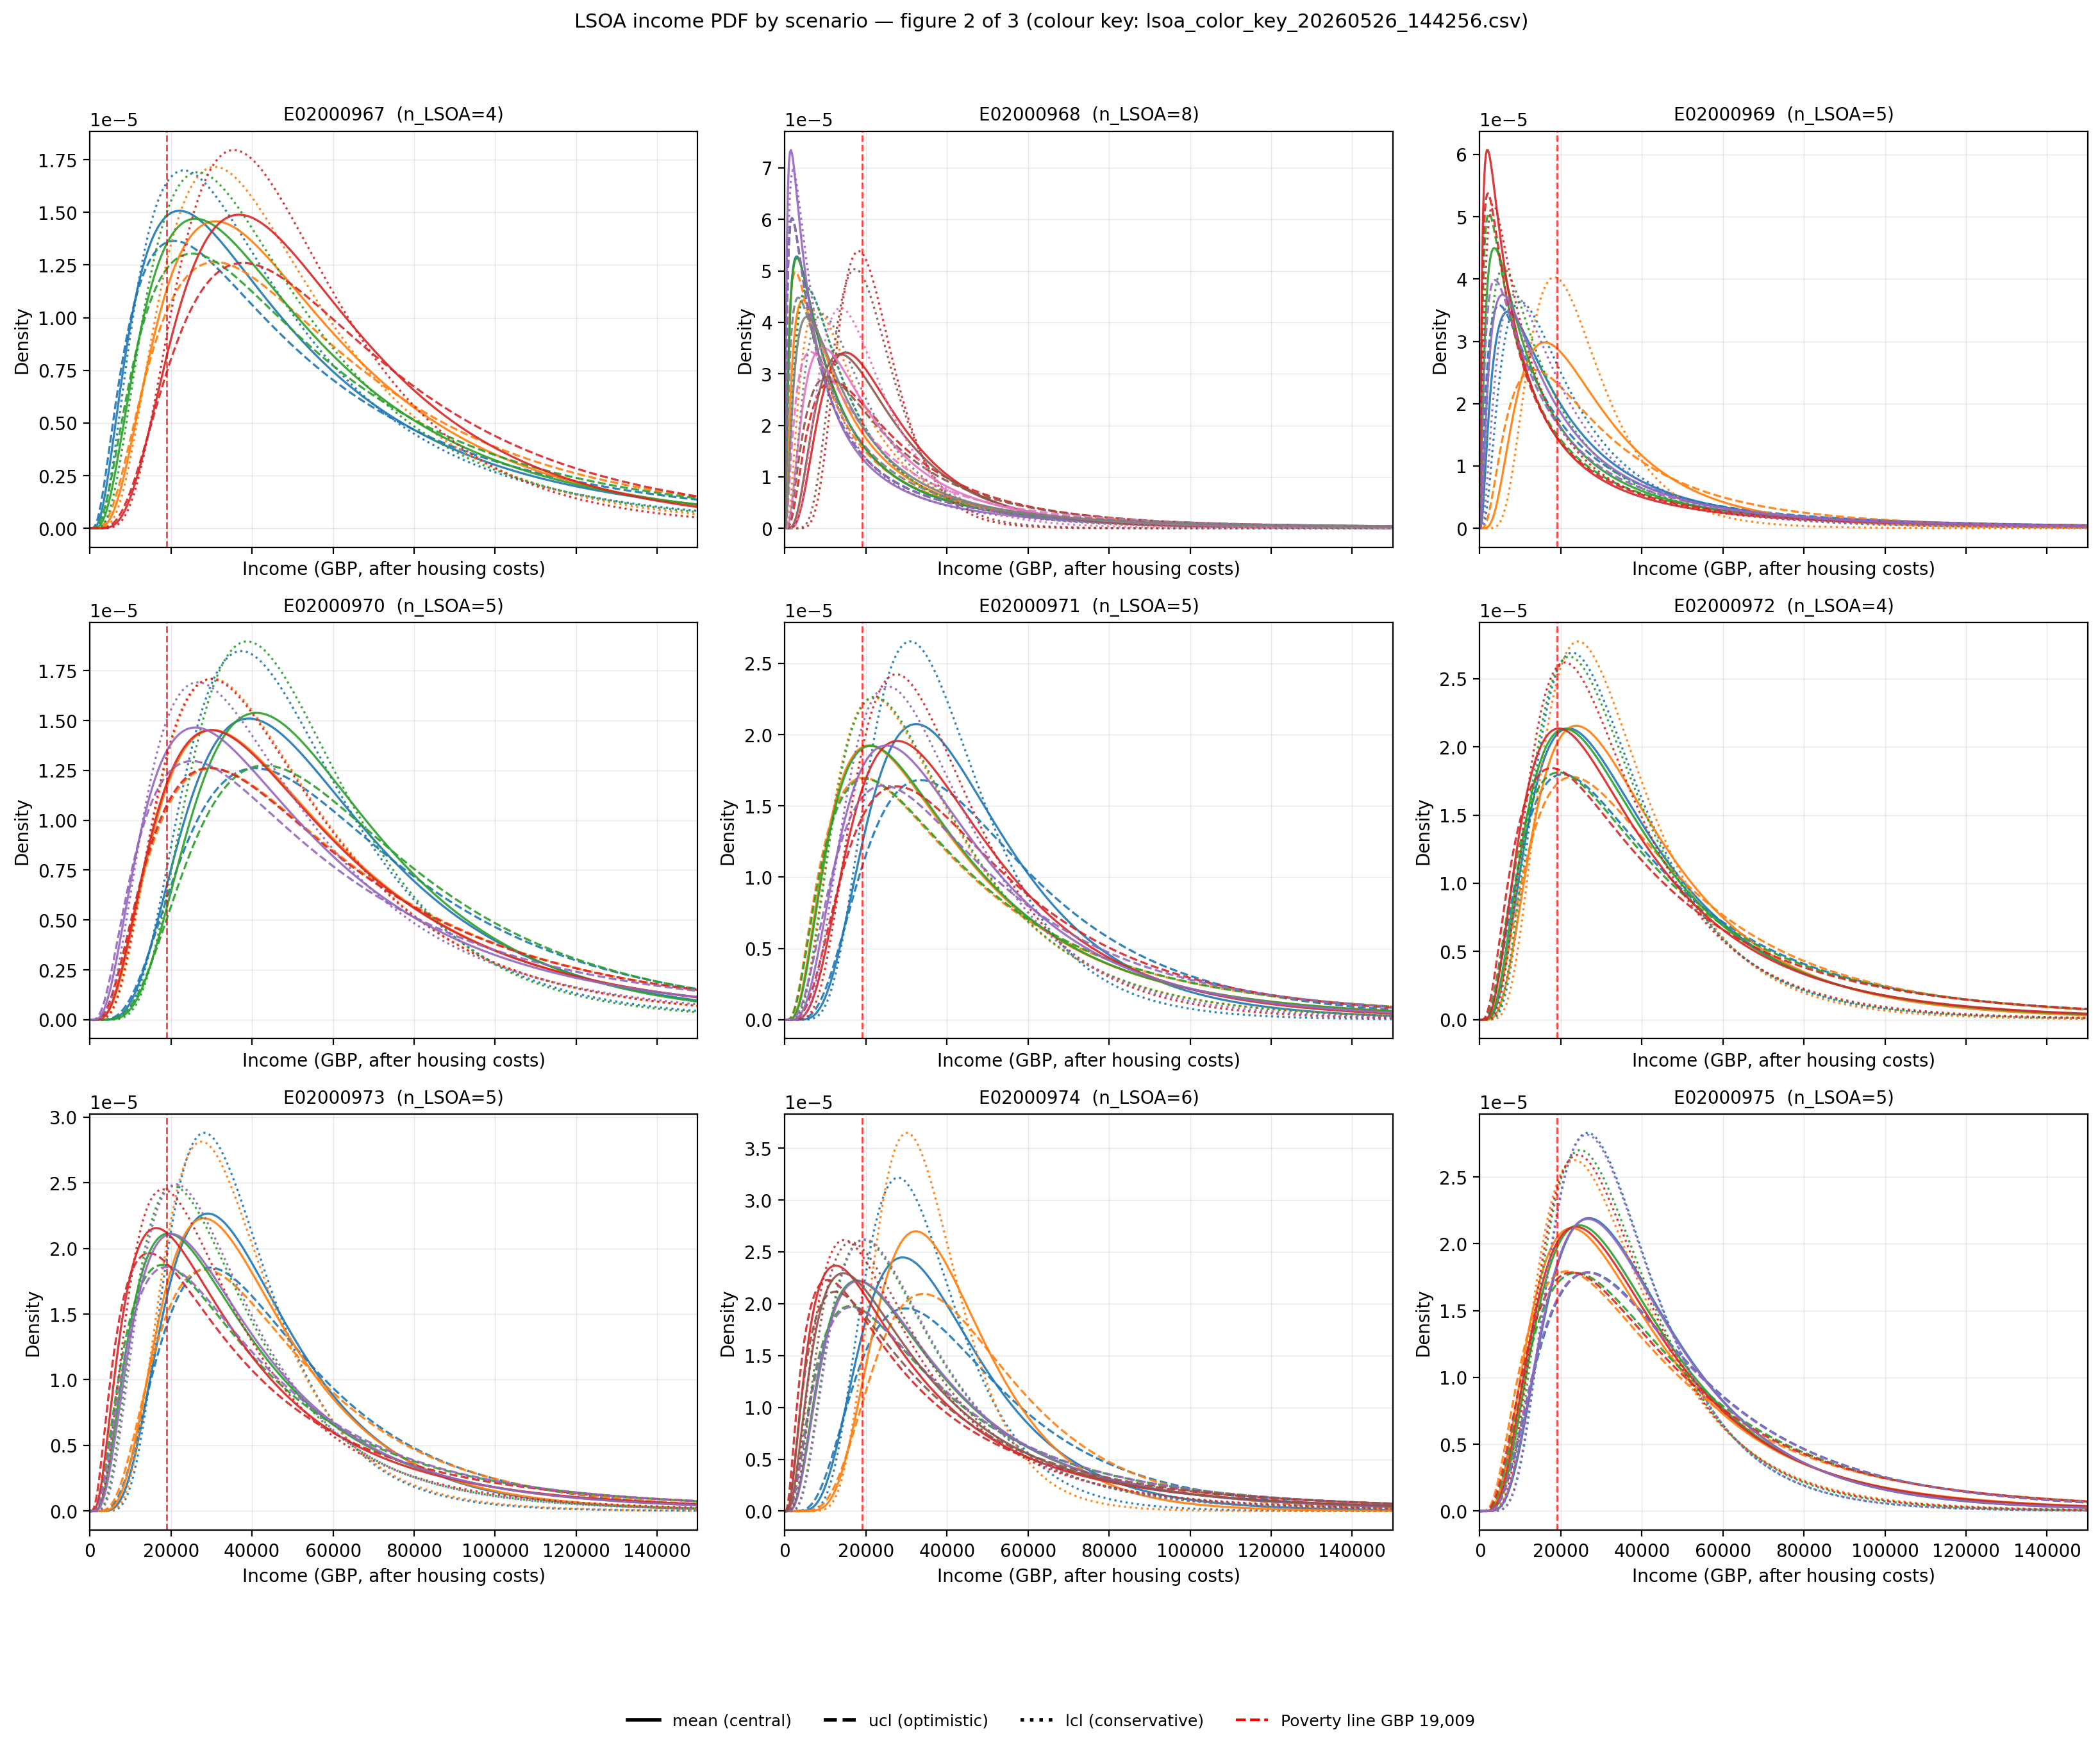
\includegraphics[width=\linewidth]{paper/figures/baseline_income_pdf_scenarios_2.png}
\caption{LSOA income PDF scenario sensitivity, panel set 2 of 3. The figure continues the diagnostic comparison of income-anchor uncertainty across Westminster MSOAs and should be interpreted as a baseline burden-modelling input rather than an observed household income distribution.}
\label{fig:lsoa-income-pdf-scenarios-2}
\end{figure}

\begin{figure}[H]
\centering
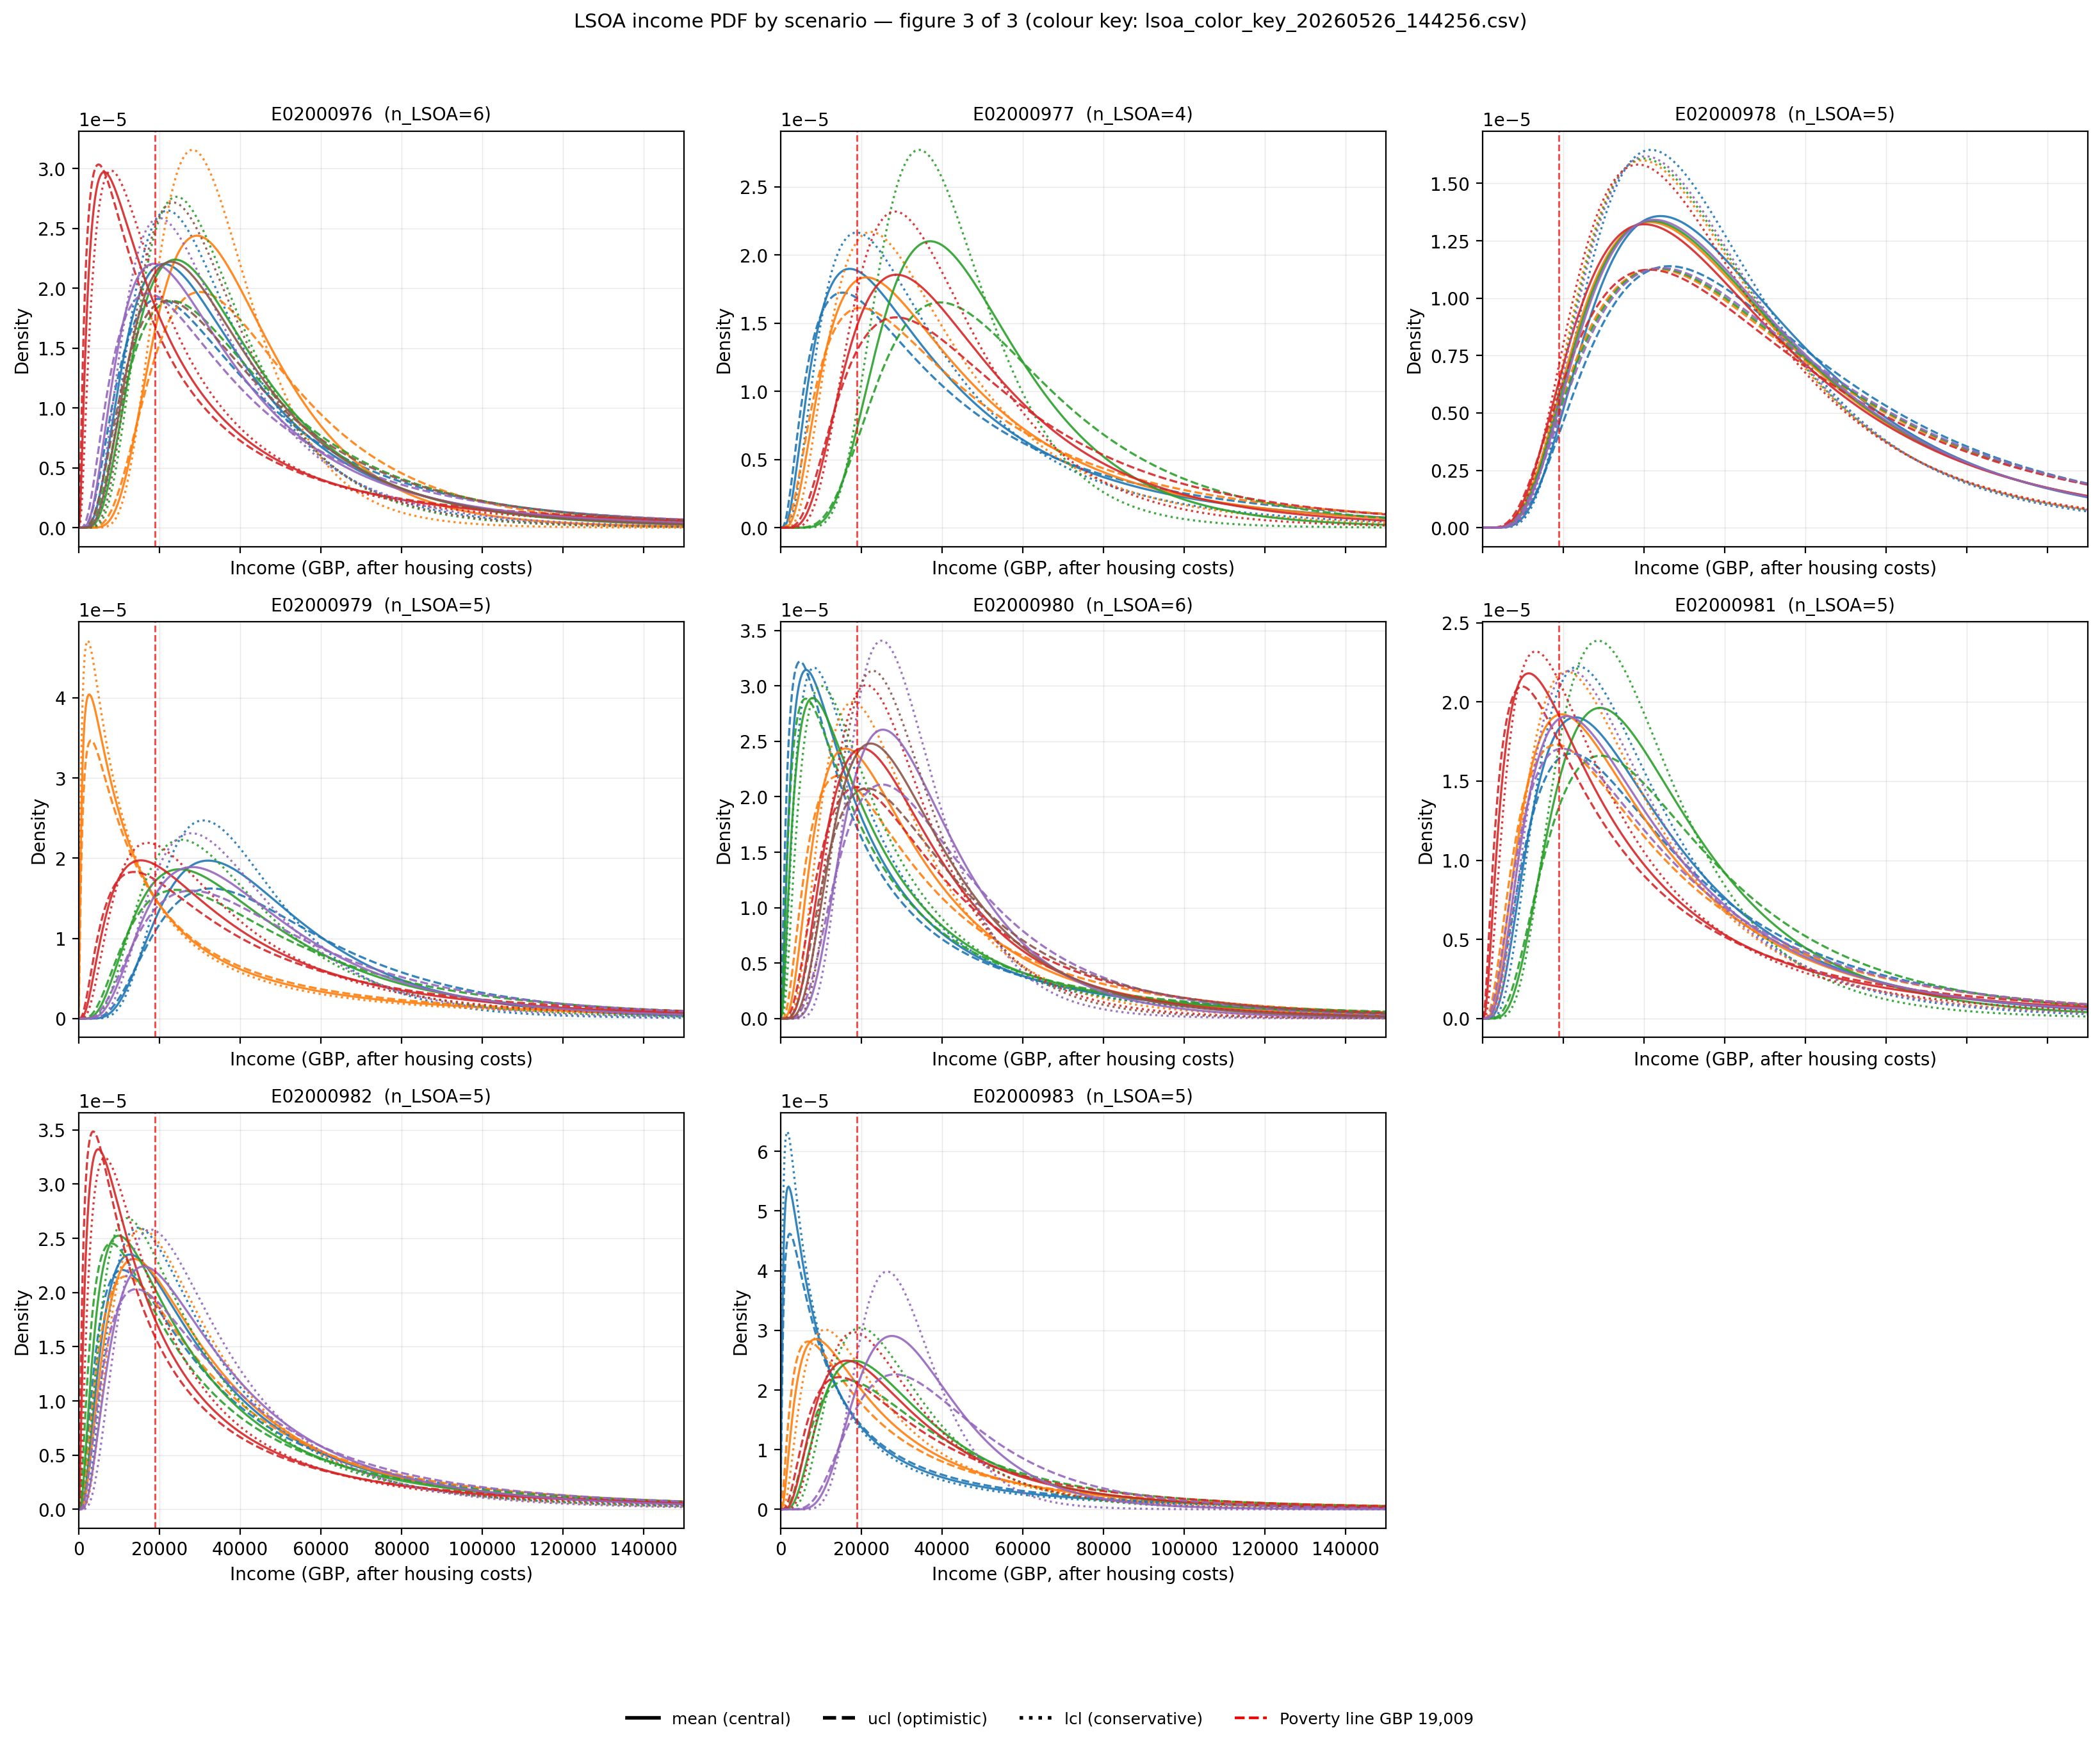
\includegraphics[width=\linewidth]{paper/figures/baseline_income_pdf_scenarios_3.png}
\caption{LSOA income PDF scenario sensitivity, panel set 3 of 3. The panels show that income-anchor uncertainty shifts selected lower-tail distributions, while the residual modelled-versus-official fuel-poverty gap remains a construct-alignment limitation rather than a price-risk result.}
\label{fig:lsoa-income-pdf-scenarios-3}
\end{figure}

\subsection{Implemented Baseline-Cost Sensitivity Outputs}

The energy-cost price-structure sensitivity archive adds a second baseline diagnostic: whether current high-burden rankings depend on the cost definition used before price shocks are introduced. The archive compares SAP-inverse required cost, EPC heating plus hot water plus lighting component cost, an exploratory unit-price-only reconstruction, and a unit-plus-standing reconstruction. It is explicitly a baseline-cost sensitivity exercise, not a final household fuel price risk model.

The main result is that baseline cost definition materially affects current exposure rankings. SAP-inverse cost has a median of \pounds 1,045 per year and a mean of \pounds 1,256 per year, while the EPC component total has a median of \pounds 651 per year and a mean of \pounds 805 per year. The median EPC-component-to-SAP-inverse cost ratio is 0.566, and 89.2 percent of properties have an EPC component cost below the SAP-inverse cost. The two measures remain correlated, with Pearson correlation 0.713 and Spearman correlation 0.763, but the top-decile high-burden groups overlap only partially: the Jaccard overlap is 0.351 for the top 10 percent and 0.449 for the top 20 percent.

Figure~\ref{fig:sap-epc-cost-scatter} visualises this divergence. It should be interpreted as a robustness warning about translating EPC/SAP information into required annual cost. The EPC component measure excludes cooking and other services implicit in the SAP-inverse total-cost measure, so the figure does not prove that one metric is universally superior. It shows that the paper's exposure rankings depend partly on the baseline-cost boundary selected before price-shock scenarios are introduced.

\begin{figure}[H]
\centering
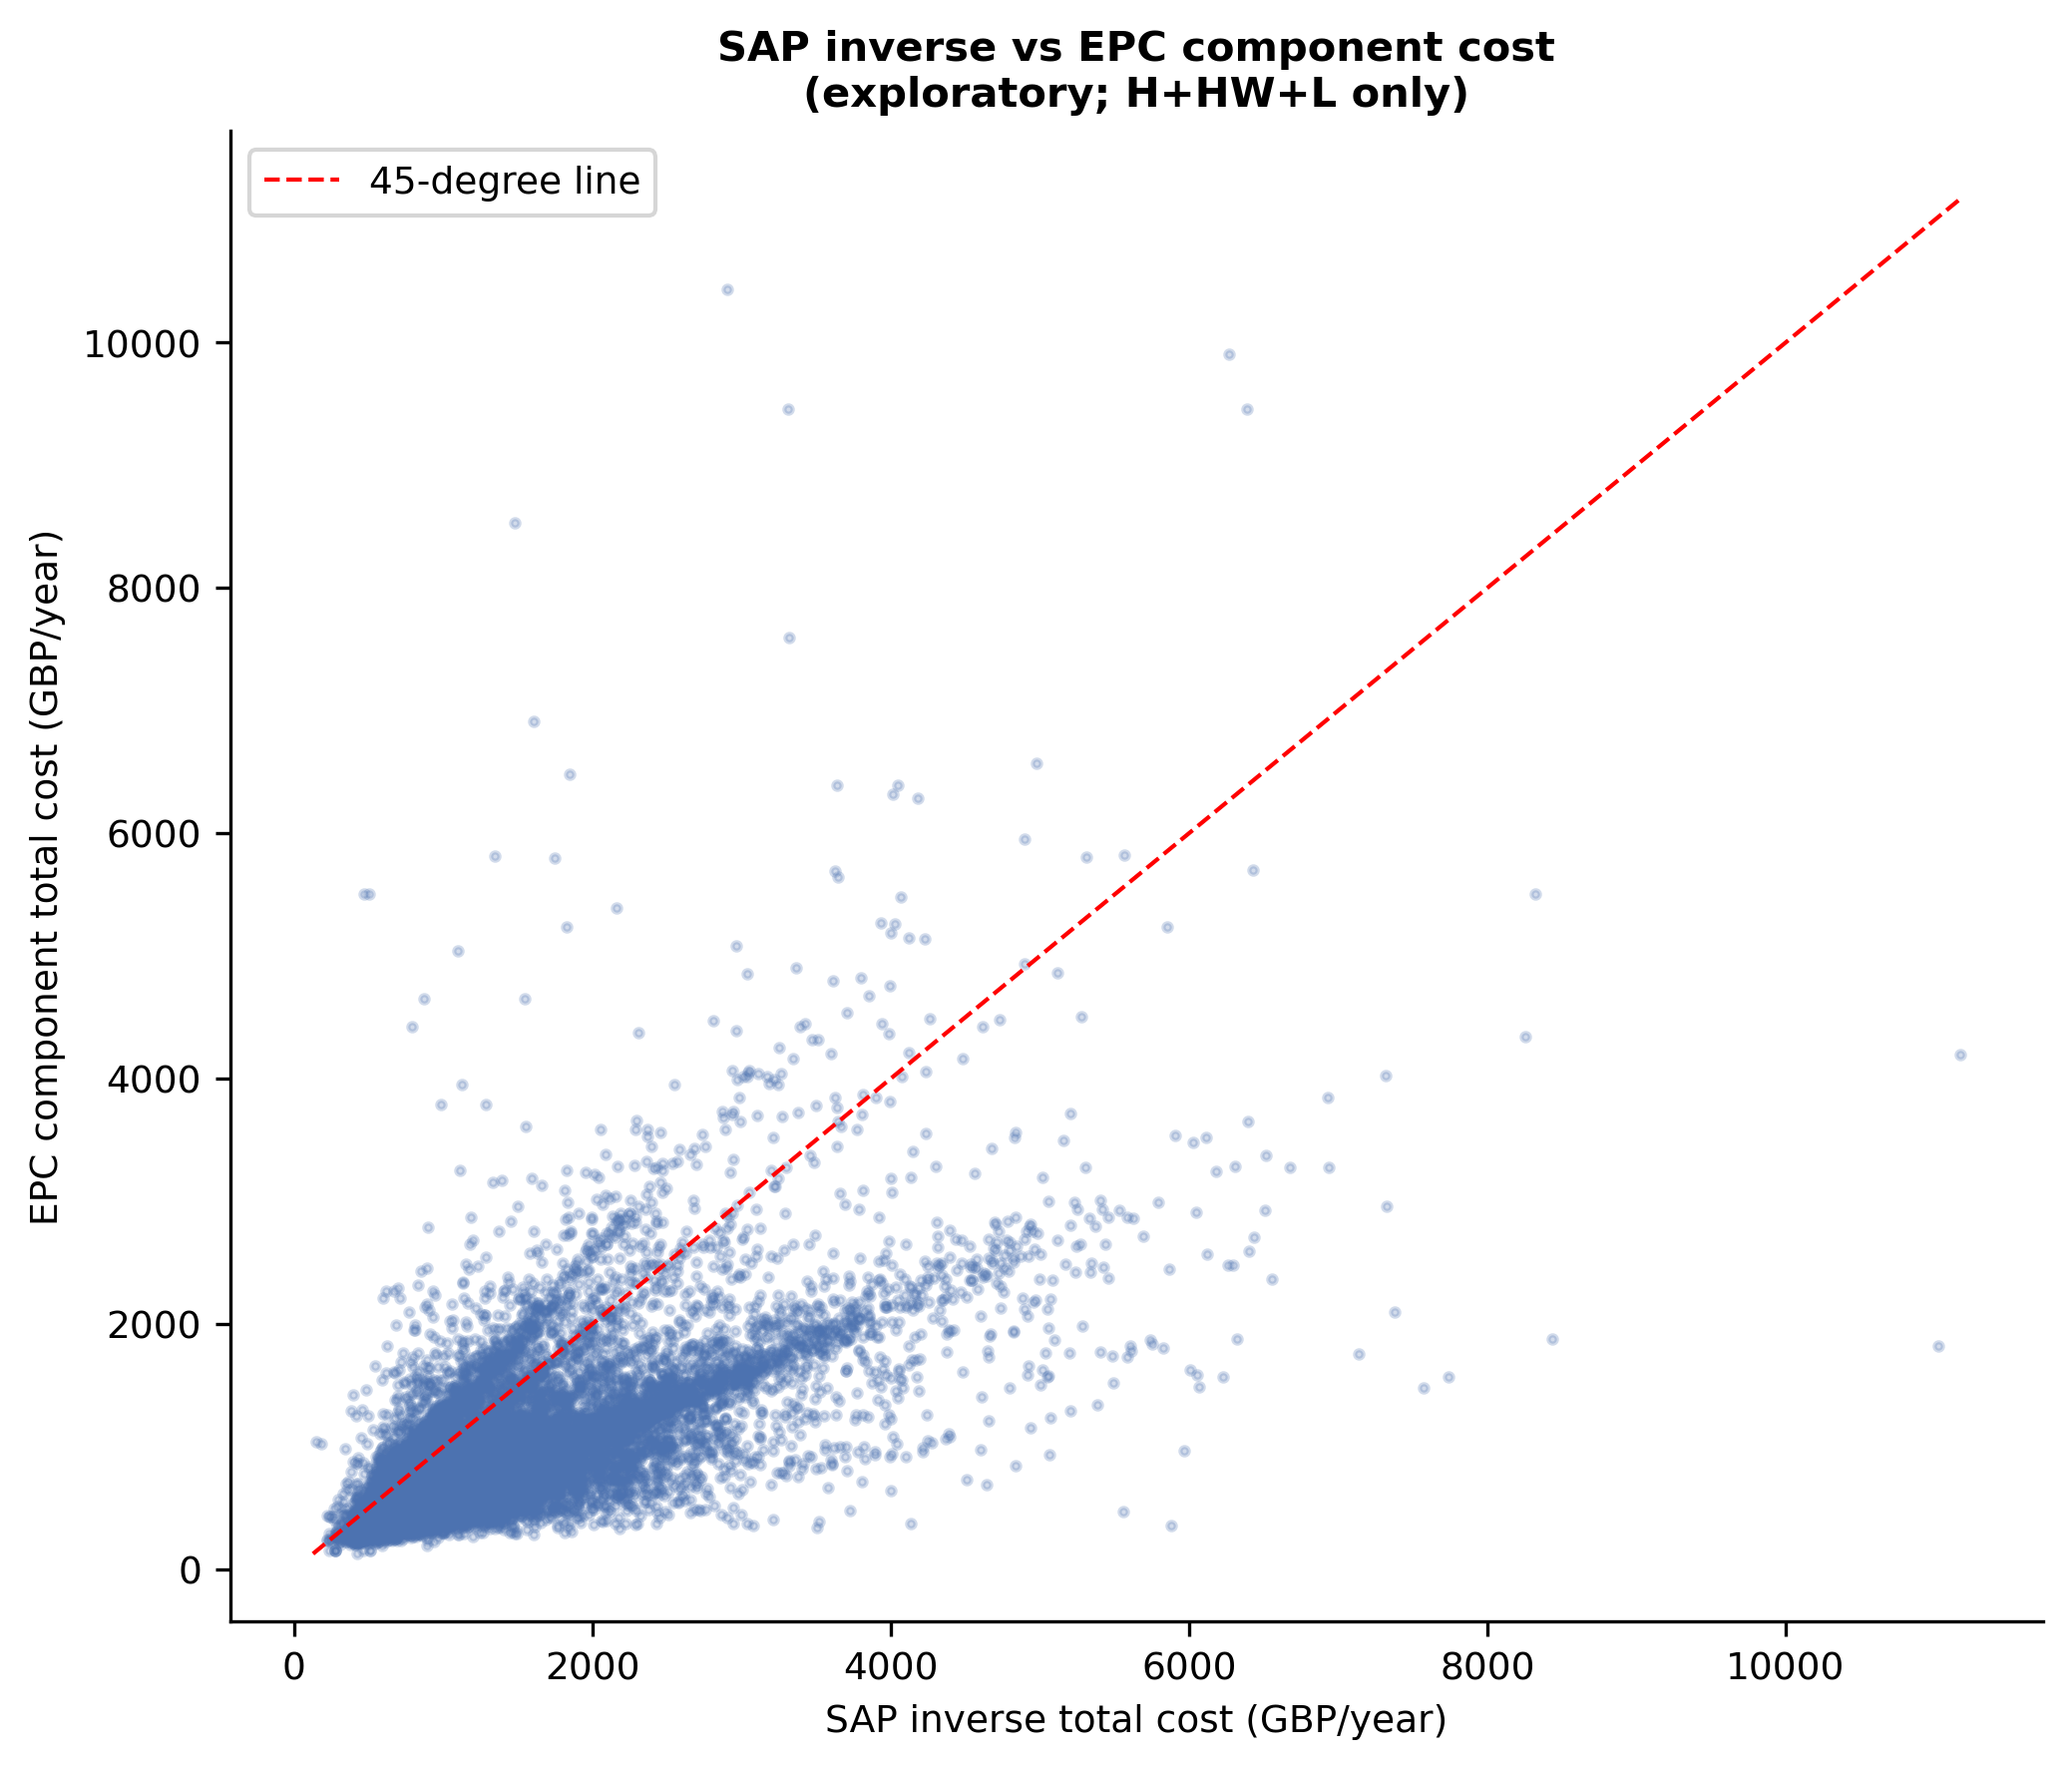
\includegraphics[width=0.88\linewidth]{paper/figures/sap_vs_epc_component_cost_scatter.png}
\caption{SAP-inverse total cost versus EPC heating, hot water, and lighting component cost in the Westminster property-level sample. The scatter shows that alternative translations from EPC/SAP information into required annual cost produce materially different baseline-cost levels and high-burden rankings; the EPC component total excludes cooking and is used here as an exploratory robustness comparator.}
\label{fig:sap-epc-cost-scatter}
\end{figure}

The standing-charge decomposition adds a more specific price-structure diagnostic. Under the current reconstruction, adding standing charges raises burden levels modestly but does not materially reorder the highest-burden decile: the median uplift is about 0.0021 burden units, and the top-decile overlap between the unit-price-only and unit-plus-standing burden measures has a Jaccard value of 0.966. Figure~\ref{fig:standing-burden-uplift-property-type} shows that property-type differentiation in this standing-charge uplift is limited in the current run. This should not be read as evidence that standing charges are unimportant. It means that a full price-shock engine should model standing charges, unit rates, off-peak or dual-tariff structures, electricity/gas price ratios, and policy mitigation separately rather than multiplying a single total-cost scalar.

\begin{figure}[H]
\centering
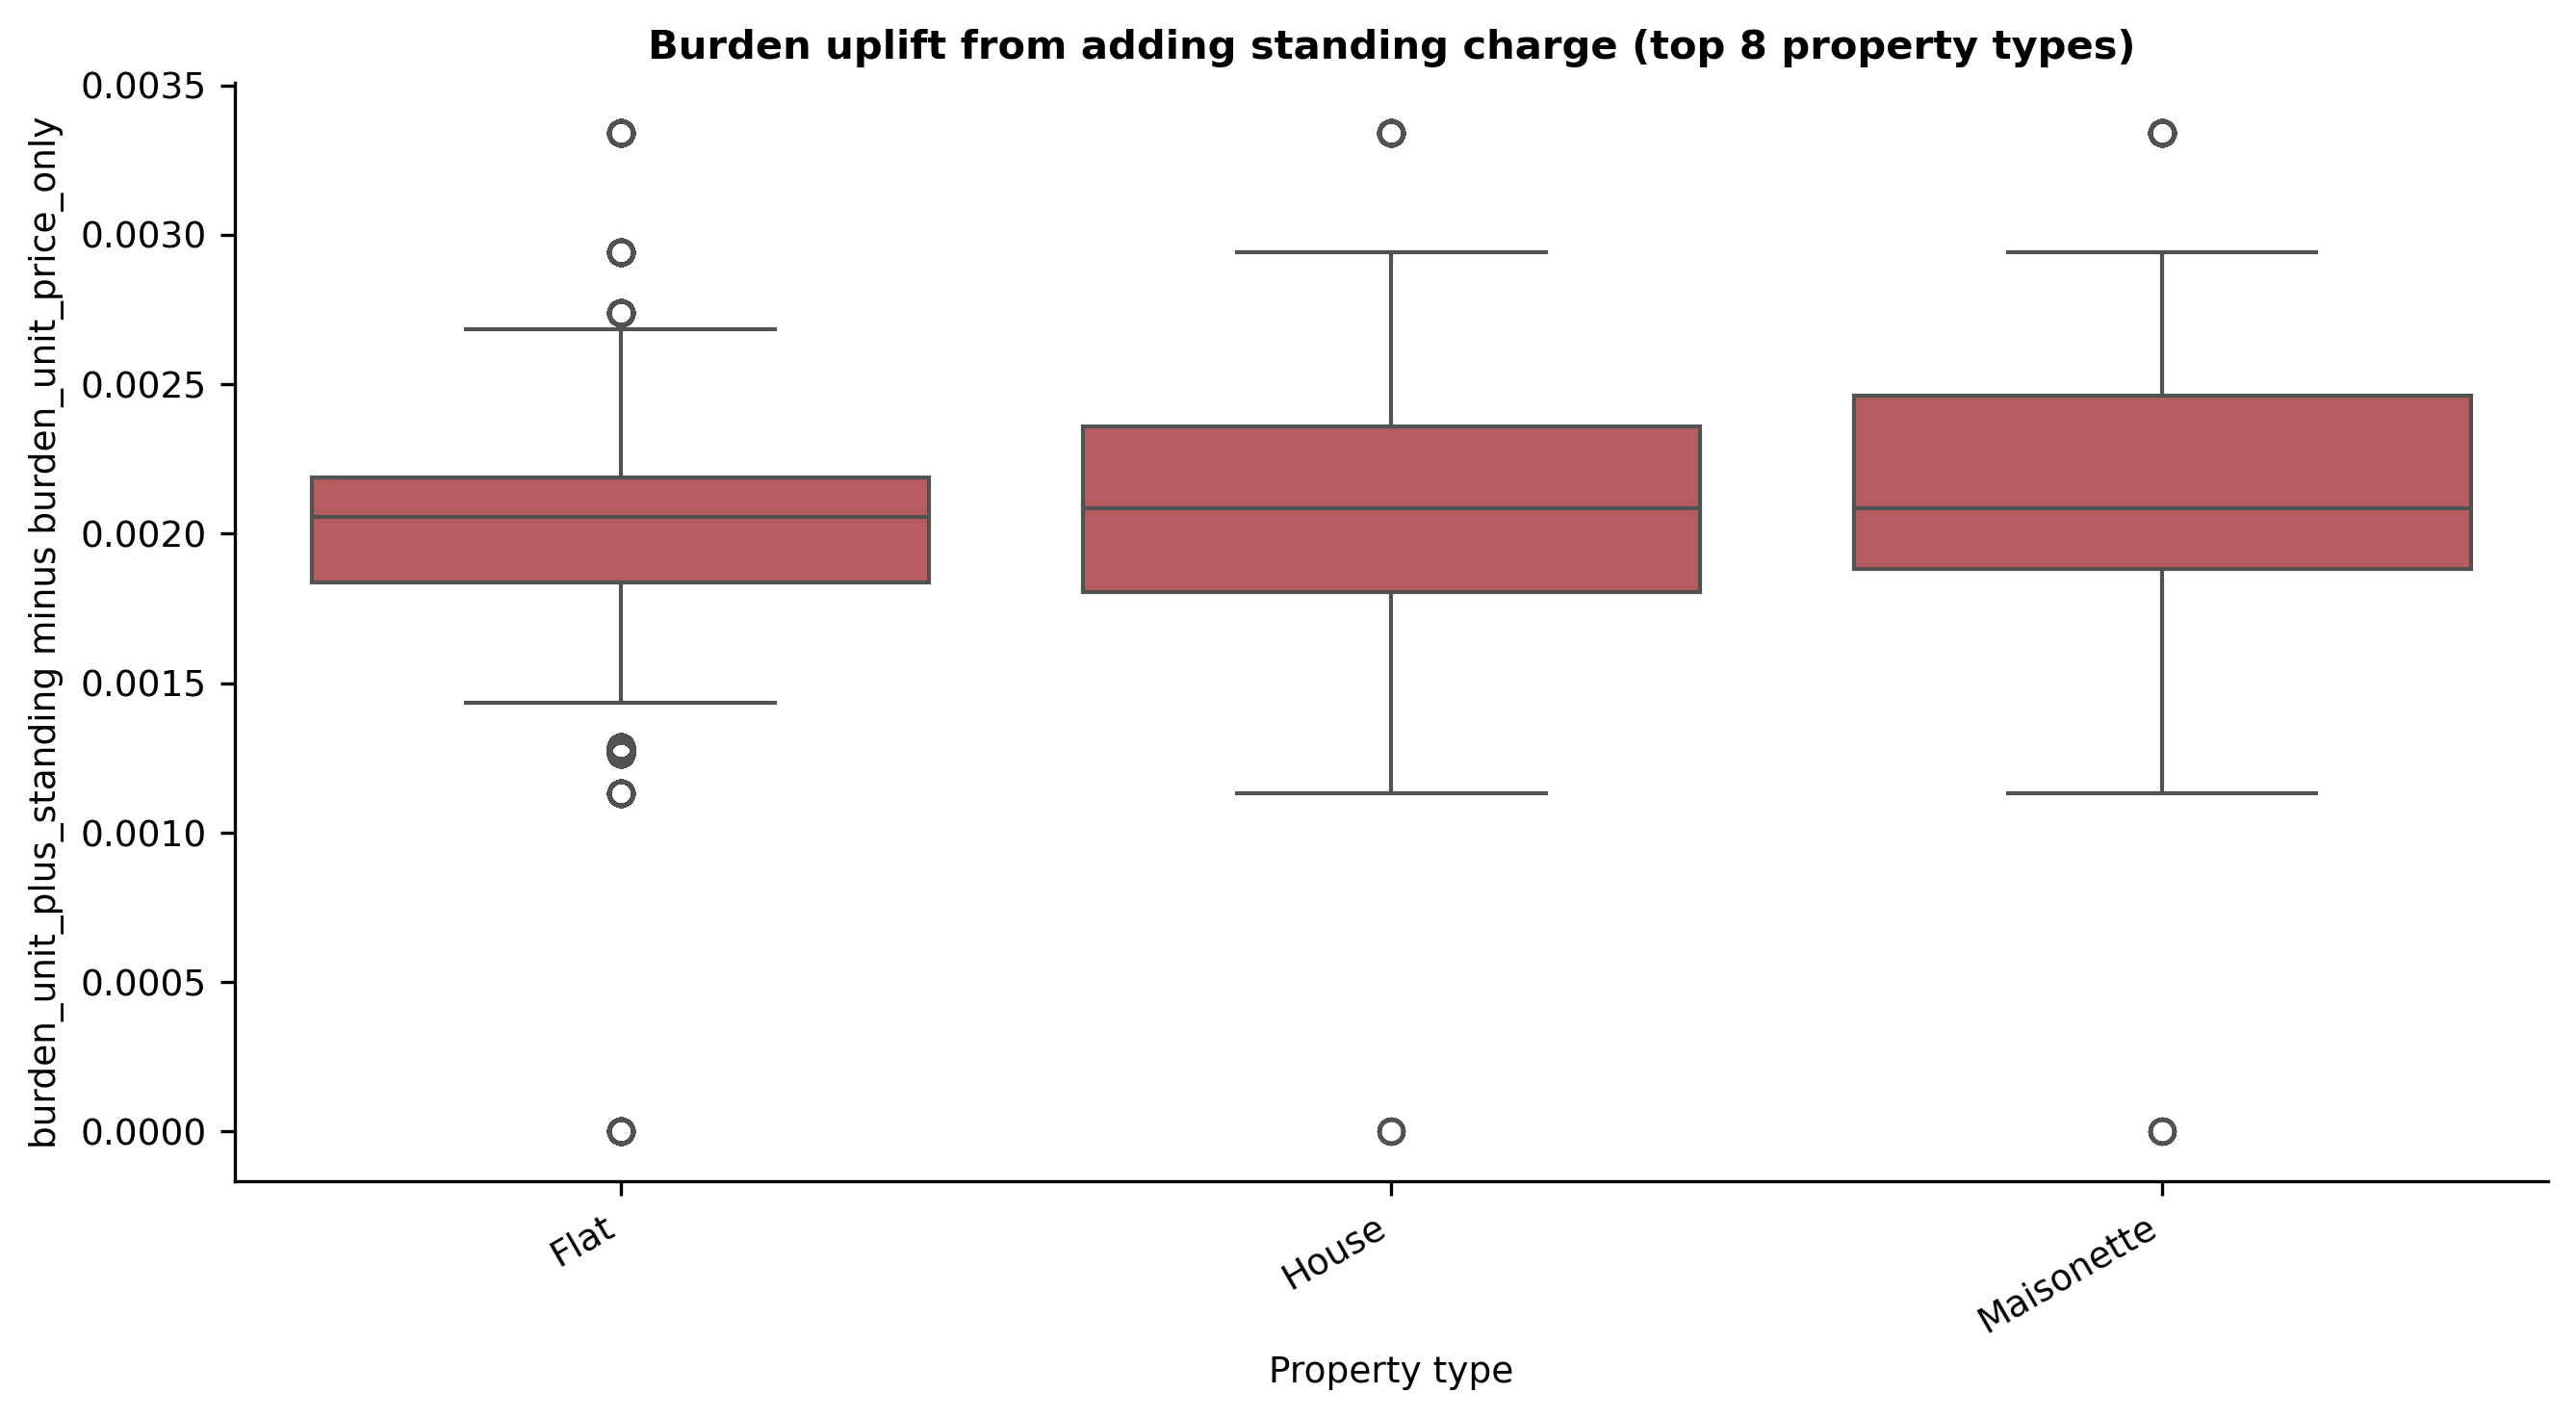
\includegraphics[width=0.82\linewidth]{paper/figures/burden_uplift_from_standing_by_property_type.png}
\caption{Burden uplift associated with adding the standing-charge component by property type. The figure reports an exploratory decomposition using MSOA point income and SAP 10.2 fuel-price mapping; it indicates modest burden-level uplift and limited property-type differentiation in this run, rather than a full standing-charge shock result.}
\label{fig:standing-burden-uplift-property-type}
\end{figure}

\subsection{Implemented High-Risk Explanation Outputs}

The latest high-risk explanation stage adds an audited EPC-enriched stock and a descriptive pathway typology. The enriched master retains 124,980 Westminster property records. After corrected UPRN standardisation, the QA workbook reports a complete match between the master properties and EPC certificate records, with zero unmatched master rows. The corrected EPC tenure proxy distributes the stock into 58,744 private rented properties, 43,686 owner-occupied properties, 20,066 social rented properties, and 2,484 unknown-tenure properties. These tenure categories are analytical proxies and should be interpreted as adaptive-capacity and governance indicators rather than as verified household tenure records.

The implemented high-risk groups remain exploratory and model-based. HR10 contains the 12,500 properties in the top decile of the probability that required energy burden exceeds 10 percent; HR20 contains the 24,996 properties in the top quintile. The deterministic burden robustness groups contain 12,498 BR10 properties and 24,996 BR20 properties, while only 737 properties have a baseline required energy burden above 10 percent under the deterministic baseline measure. As Figure~\ref{fig:hr-br-overlap} shows, HR10 and BR10 overlap for 7,128 properties, or 57.0 percent of each group. This overlap is large enough to show that the probabilistic and deterministic indicators identify a related high-burden tail, but incomplete enough to justify reporting both.

\begin{figure}[H]
\centering
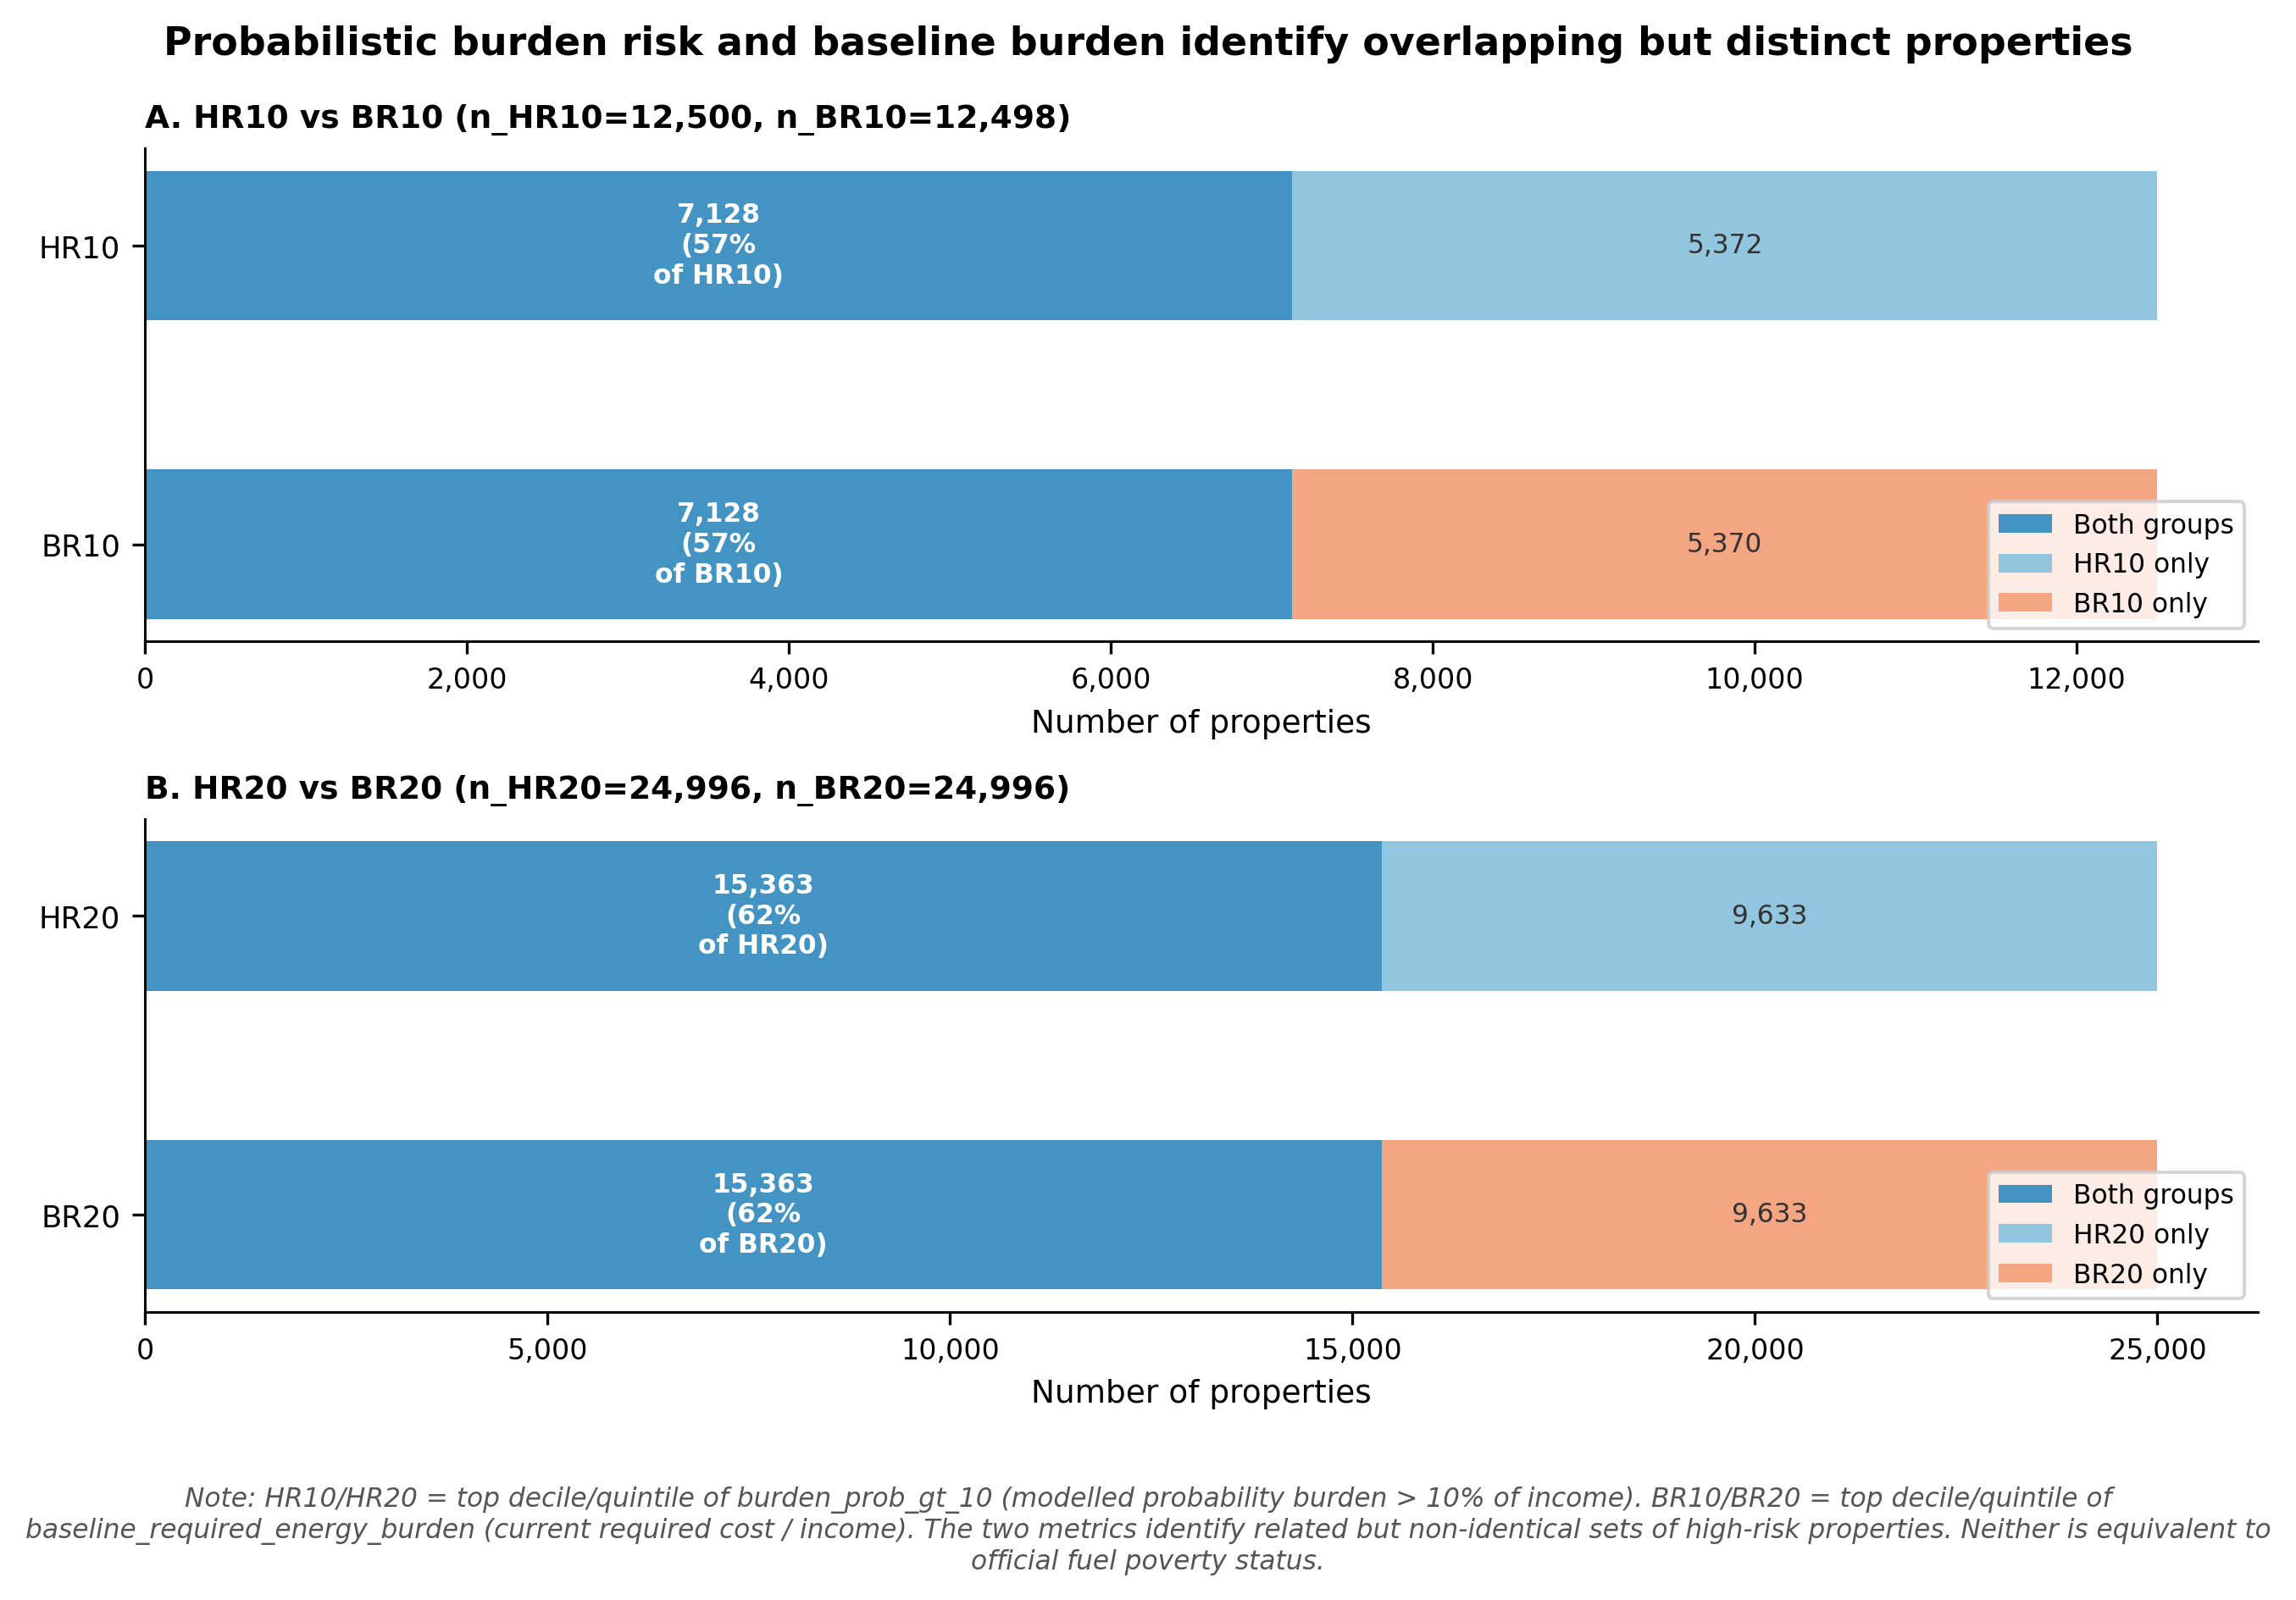
\includegraphics[width=\linewidth]{paper/figures/high_risk_hr_br_overlap.png}
\caption{Overlap between probabilistic high-risk groups (HR10/HR20) and deterministic baseline burden groups (BR10/BR20). The partial overlap shows that income-distribution exposure and deterministic burden intensity identify related but non-identical current high-burden sets.}
\label{fig:hr-br-overlap}
\end{figure}

The strongest descriptive signal in the current outputs is the interaction between dwelling size and energy performance. Figure~\ref{fig:epc-floorarea-hr10} shows that EPC E--F--G properties above 120 m$^2$ have an HR10 share of 69.68 percent and an HR20 share of 85.21 percent, with a median baseline burden of 7.26 percent. E--F--G houses also show high within-type exposure, with an HR10 share of 56.08 percent. By contrast, E--F--G flats have a lower within-type HR10 share of 19.38 percent, but remain important because flats are numerous in the Westminster stock.

\begin{figure}[H]
\centering
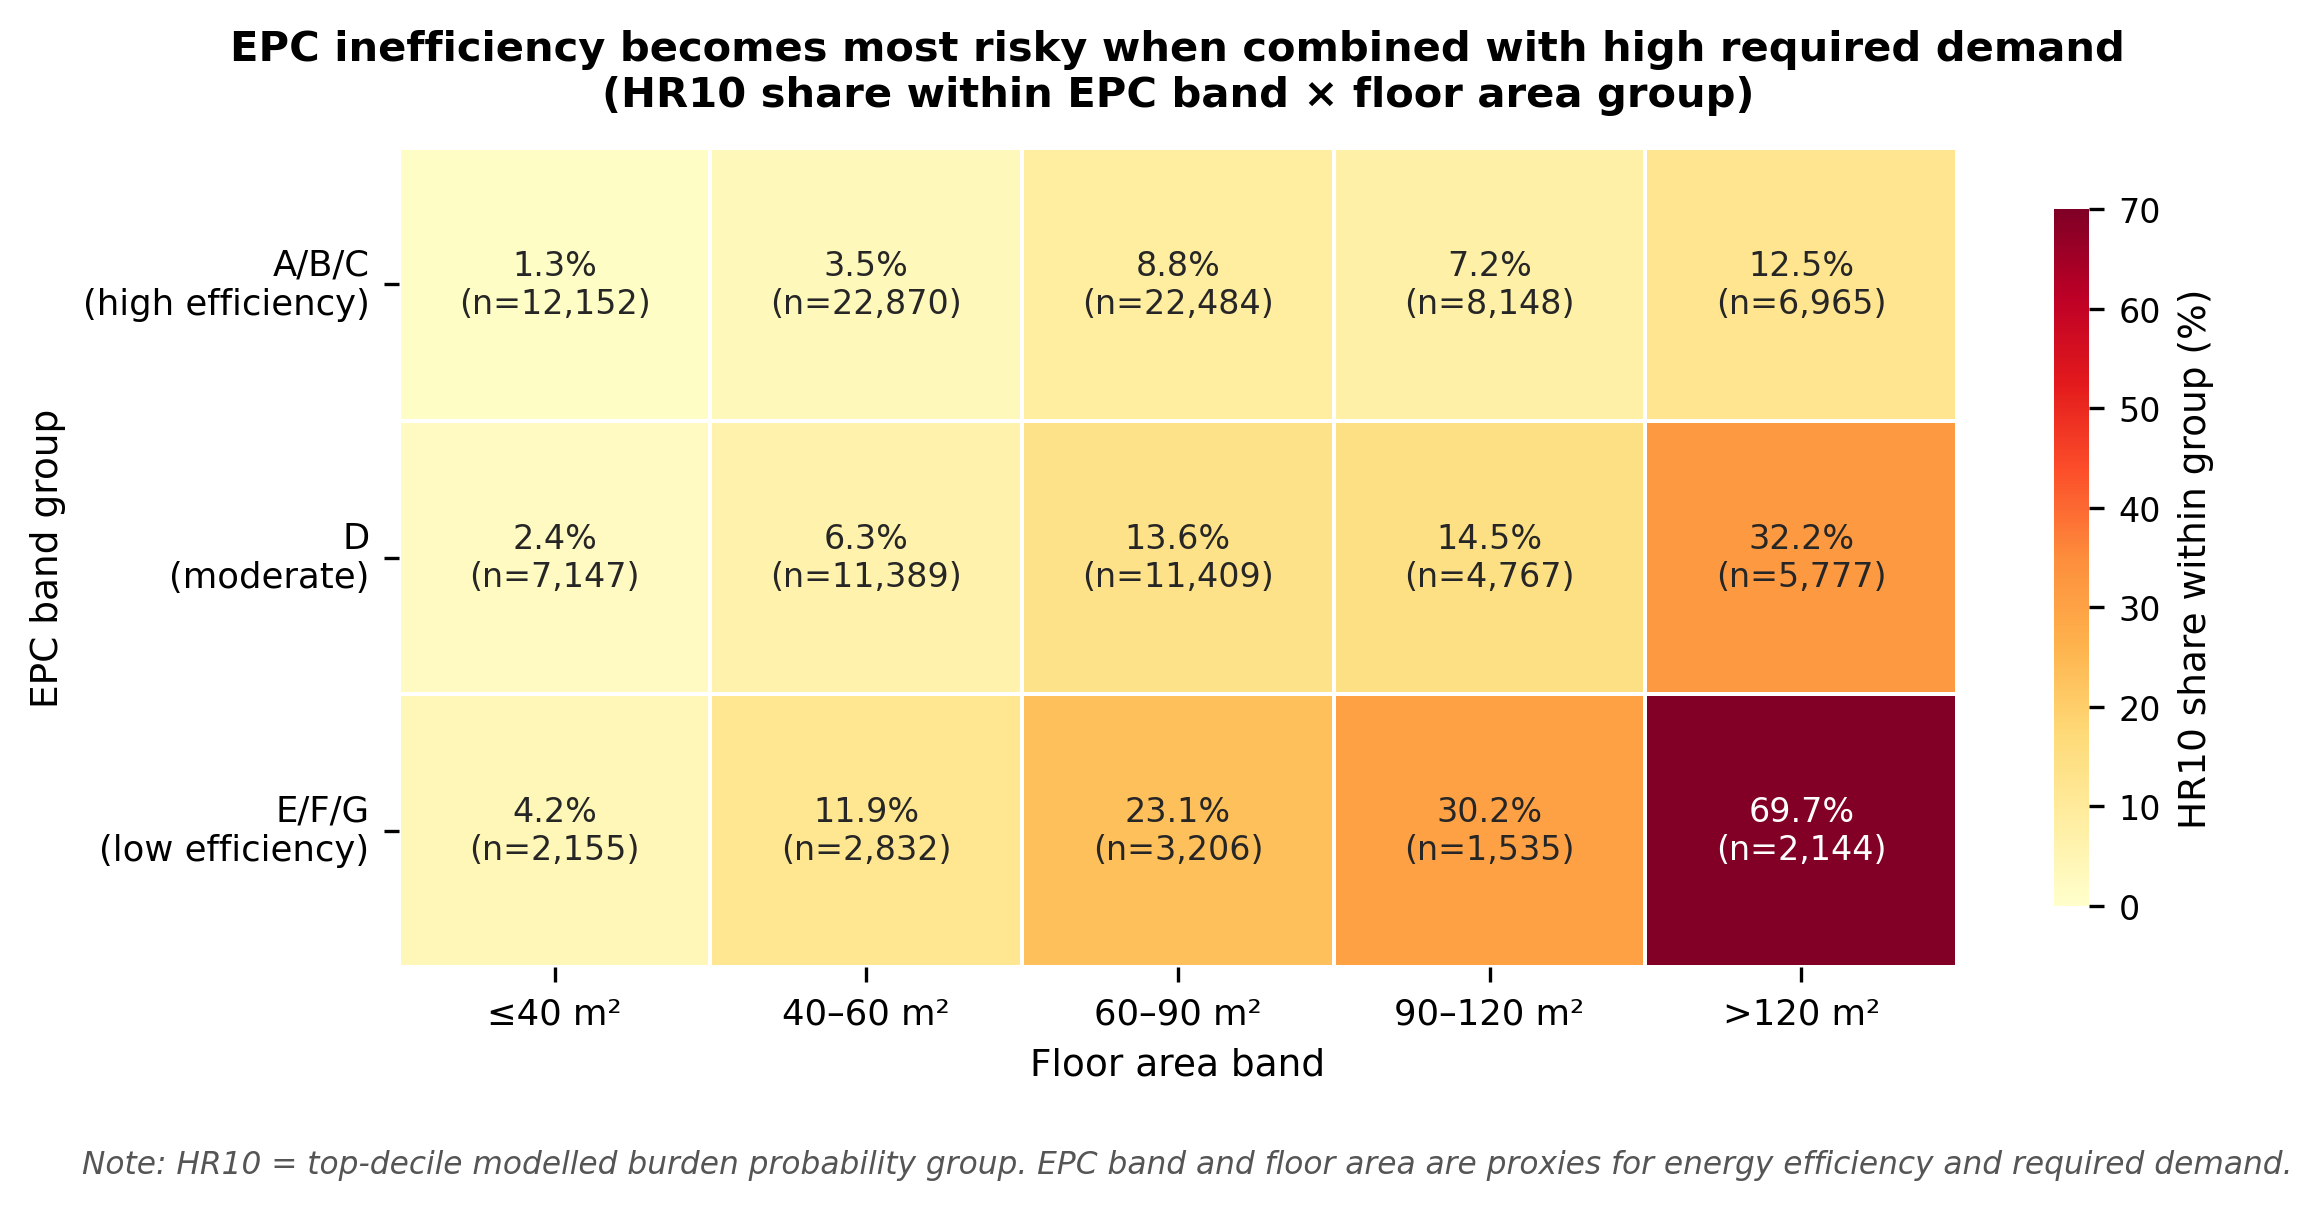
\includegraphics[width=0.86\linewidth]{paper/figures/high_risk_epc_floorarea_heatmap.png}
\caption{HR10 share by EPC band and floor-area group. The heatmap shows that low energy performance becomes most consequential where required demand is amplified by dwelling size; EPC band alone is therefore an incomplete risk signal.}
\label{fig:epc-floorarea-hr10}
\end{figure}

\begin{table}[htbp]
\centering
\footnotesize
\setlength{\tabcolsep}{3pt}
\caption{Current high-risk pathway typology from the latest explanatory run}
\label{tab:high-risk-pathways}
\begin{tabular}{>{\raggedright\arraybackslash}p{0.36\linewidth}rrrr}
\toprule
Pathway & Properties & Stock & HR10 & HR10 contrib. \\
\midrule
Inefficient large owner-occupied gas houses & 2,802 & 2.24\% & 50.25\% & 11.26\% \\
Social rented estate/block risk & 7,016 & 5.61\% & 22.66\% & 12.72\% \\
Private rented weak-fabric gas flats & 34,672 & 27.74\% & 4.18\% & 11.60\% \\
Electric-heated inefficient flats/maisonettes & 10,256 & 8.21\% & 13.83\% & 11.34\% \\
High-demand inefficient maisonettes & 2,220 & 1.78\% & 25.81\% & 4.58\% \\
Other high-risk residual group & 13,063 & 10.45\% & 46.40\% & 48.49\% \\
Not high risk / comparison stock & 54,951 & 43.97\% & 0.00\% & 0.00\% \\
\bottomrule
\end{tabular}
\end{table}

Table~\ref{tab:high-risk-pathways} should be read as a targeting and interpretation device, not as a final causal attribution model. It separates two policy-relevant rankings: the highest within-pathway risk is concentrated in inefficient large owner-occupied gas houses, high-demand inefficient maisonettes, and social rented estate/block risk, while the largest contributions to all HR10 properties come from social rented estate/block risk, private rented weak-fabric gas flats, electric-heated inefficient flats/maisonettes, and the residual high-risk group. Figure~\ref{fig:high-risk-pathway-contribution} visualises the same distinction between risk intensity and stock-scale contribution. The next empirical outputs should therefore report both rankings.

\begin{figure}[H]
\centering
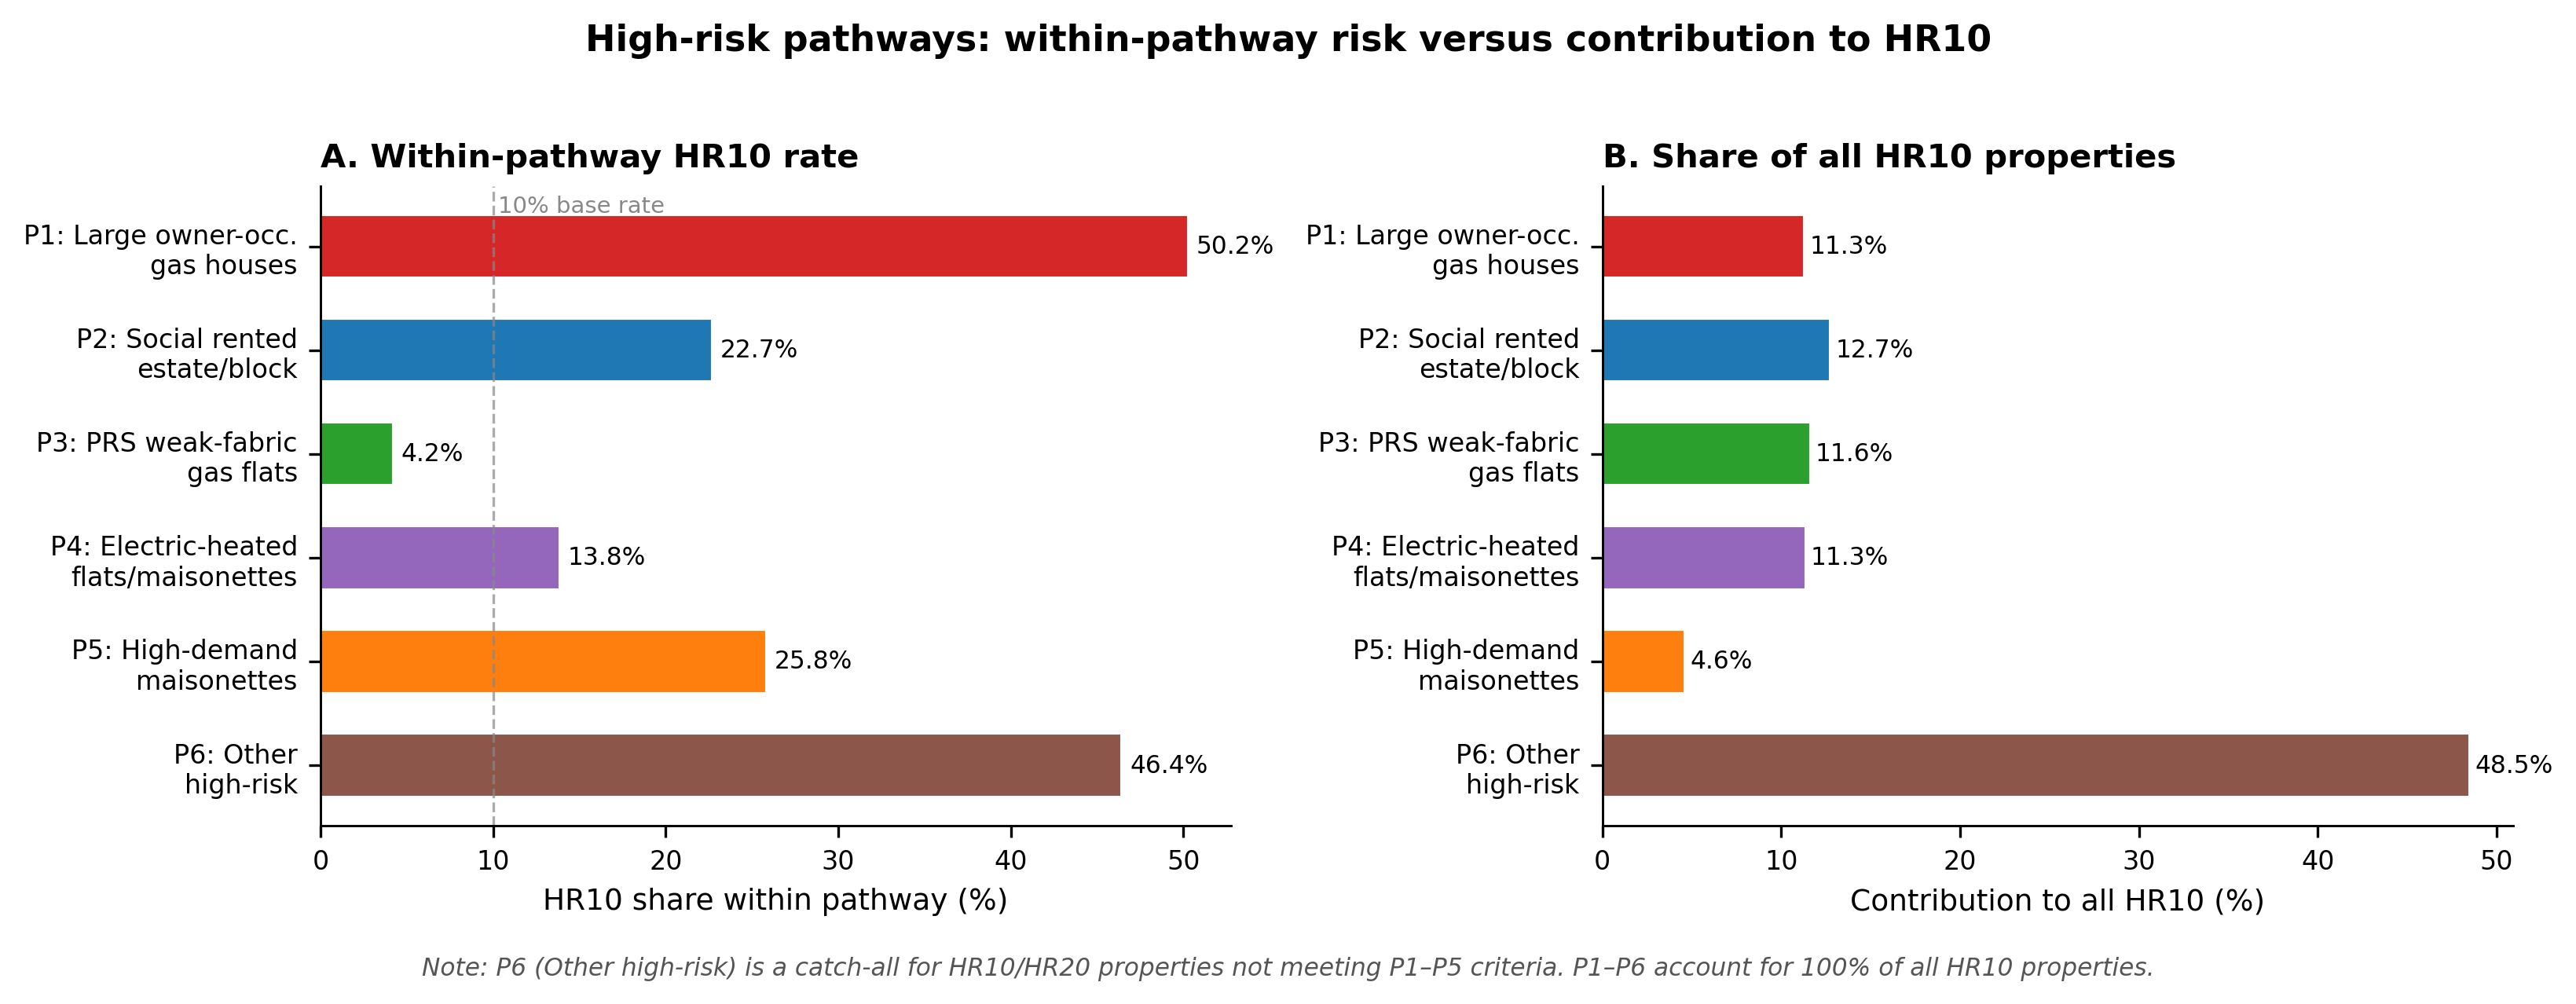
\includegraphics[width=\linewidth]{paper/figures/high_risk_pathway_contribution.png}
\caption{Within-pathway HR10 risk and contribution to all HR10 properties. The figure distinguishes intensity from scale: some pathways have high within-group exposure, while others contribute substantially because they are more numerous in the Westminster stock.}
\label{fig:high-risk-pathway-contribution}
\end{figure}

\begin{figure}[H]
\centering
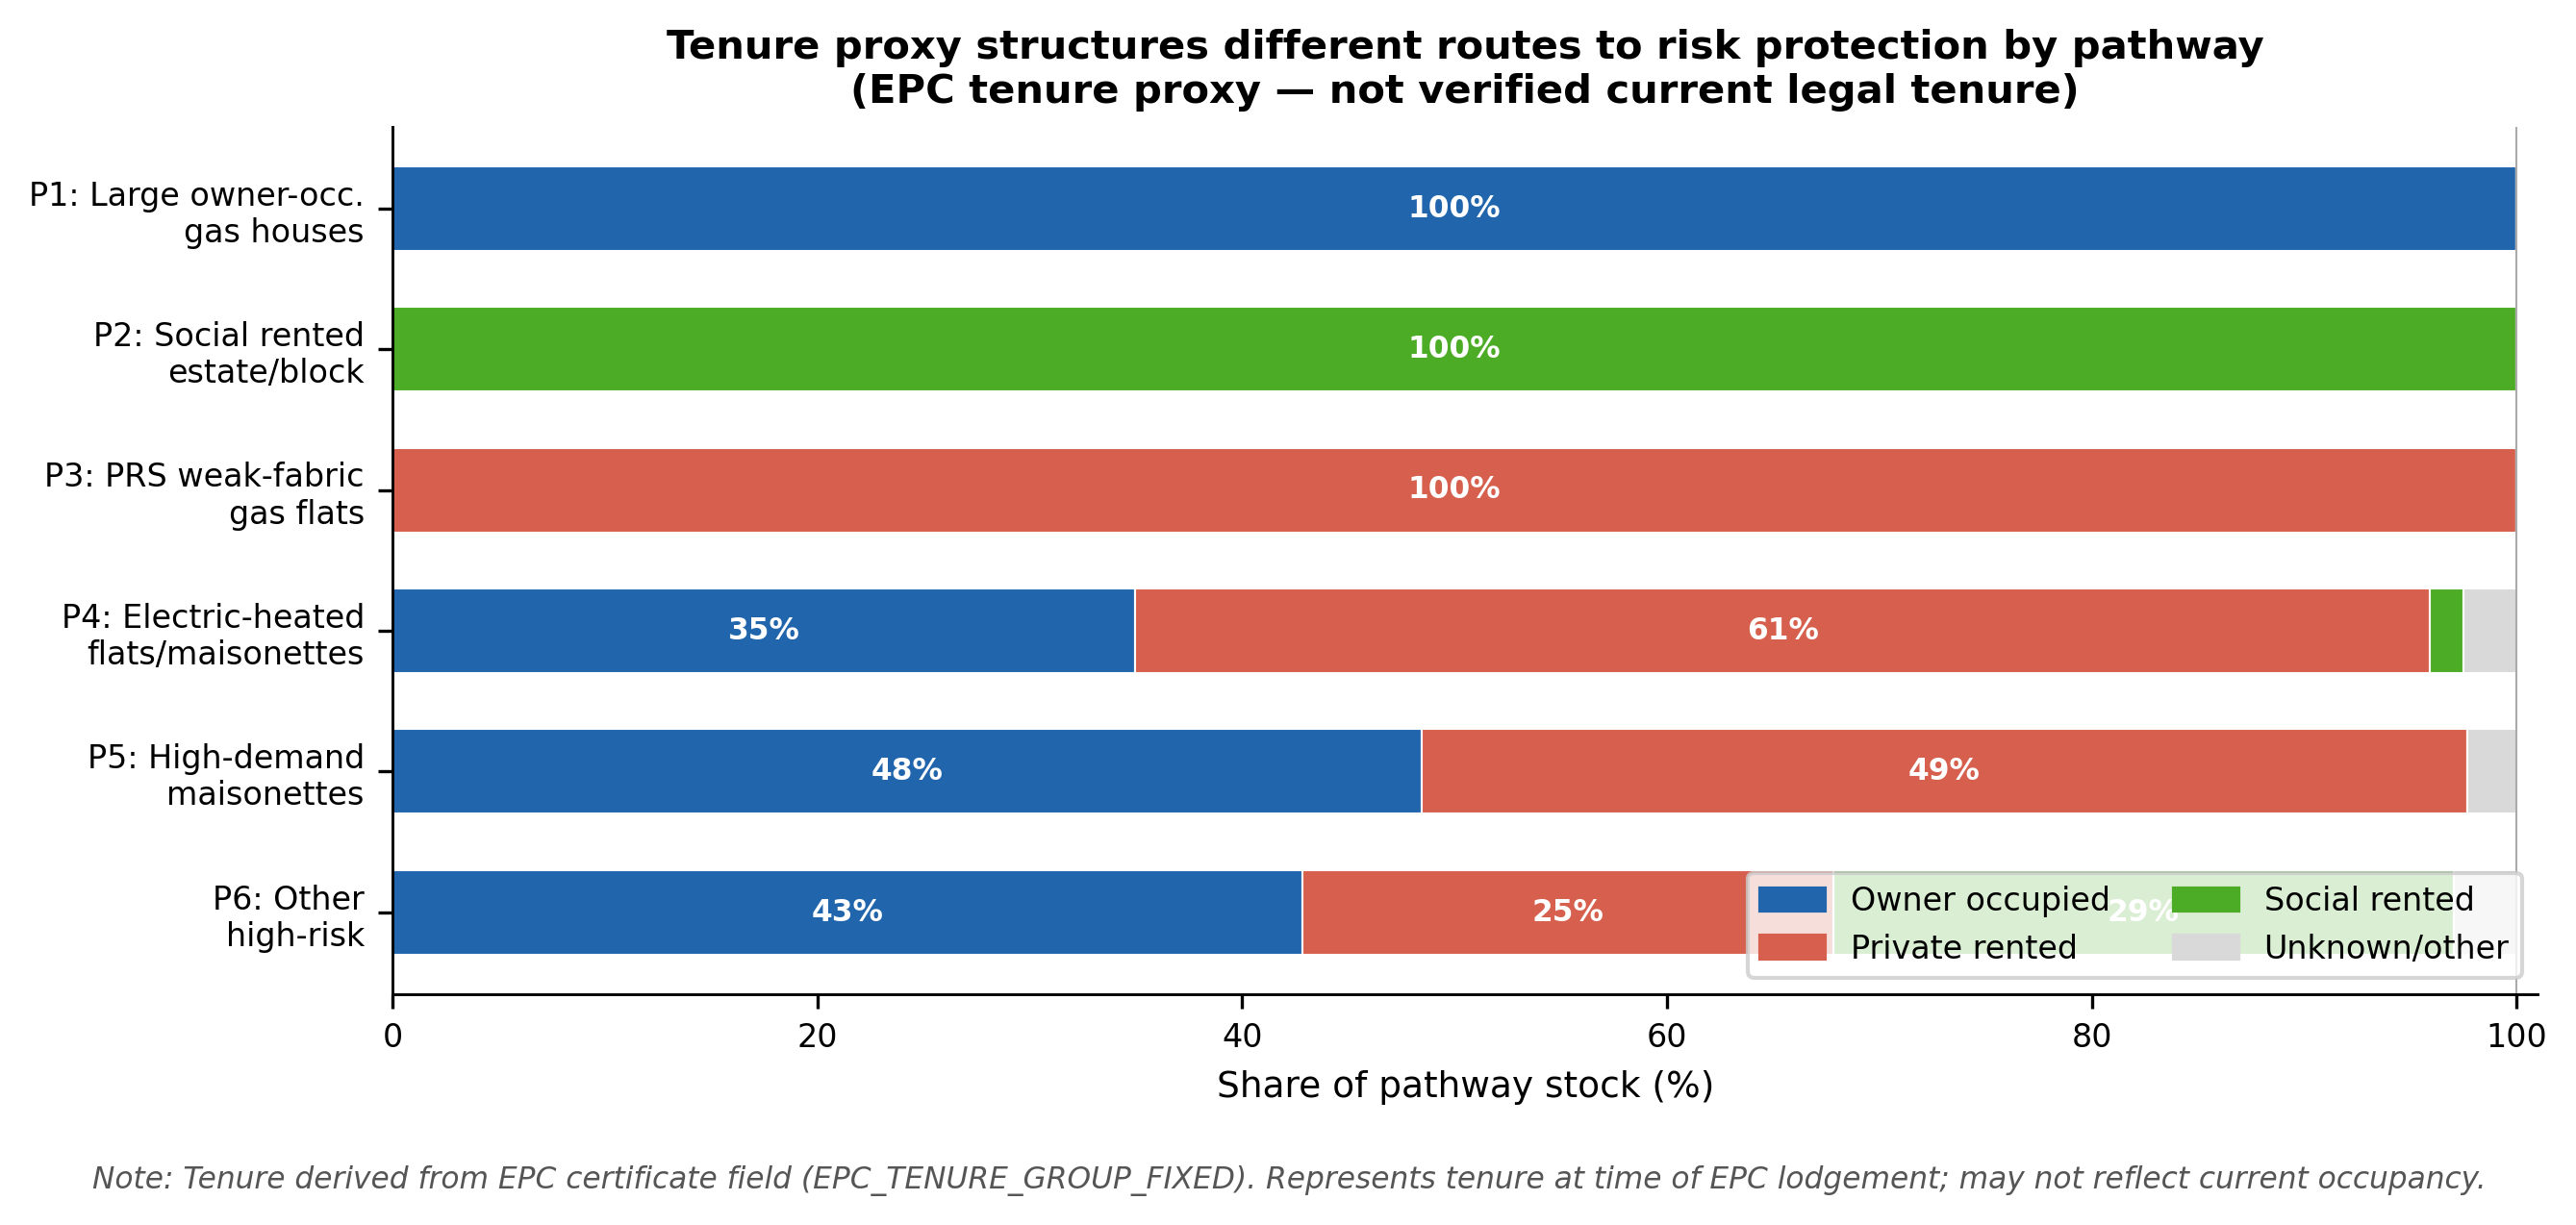
\includegraphics[width=0.92\linewidth]{paper/figures/high_risk_tenure_by_pathway.png}
\caption{Tenure-proxy composition by high-risk pathway. The figure links each descriptive pathway to a different governance route, including owner-occupation, social housing delivery, private rented enforcement, and mixed residual cases.}
\label{fig:tenure-by-pathway}
\end{figure}

Figure~\ref{fig:tenure-by-pathway} then shows why these pathways imply different governance routes, rather than a single retrofit-delivery model. The electric-exposure comparison in Figure~\ref{fig:electric-exposure} isolates inefficient flats and maisonettes with EPC-recorded electricity exposure from non-electric low-EPC comparators and the remaining stock. Its purpose is not to claim that electrification causes high burden, but to show why household-facing electricity prices, fabric quality, and tariff access must be modelled before clean heat can be interpreted as price-risk protection.

\begin{figure}[H]
\centering
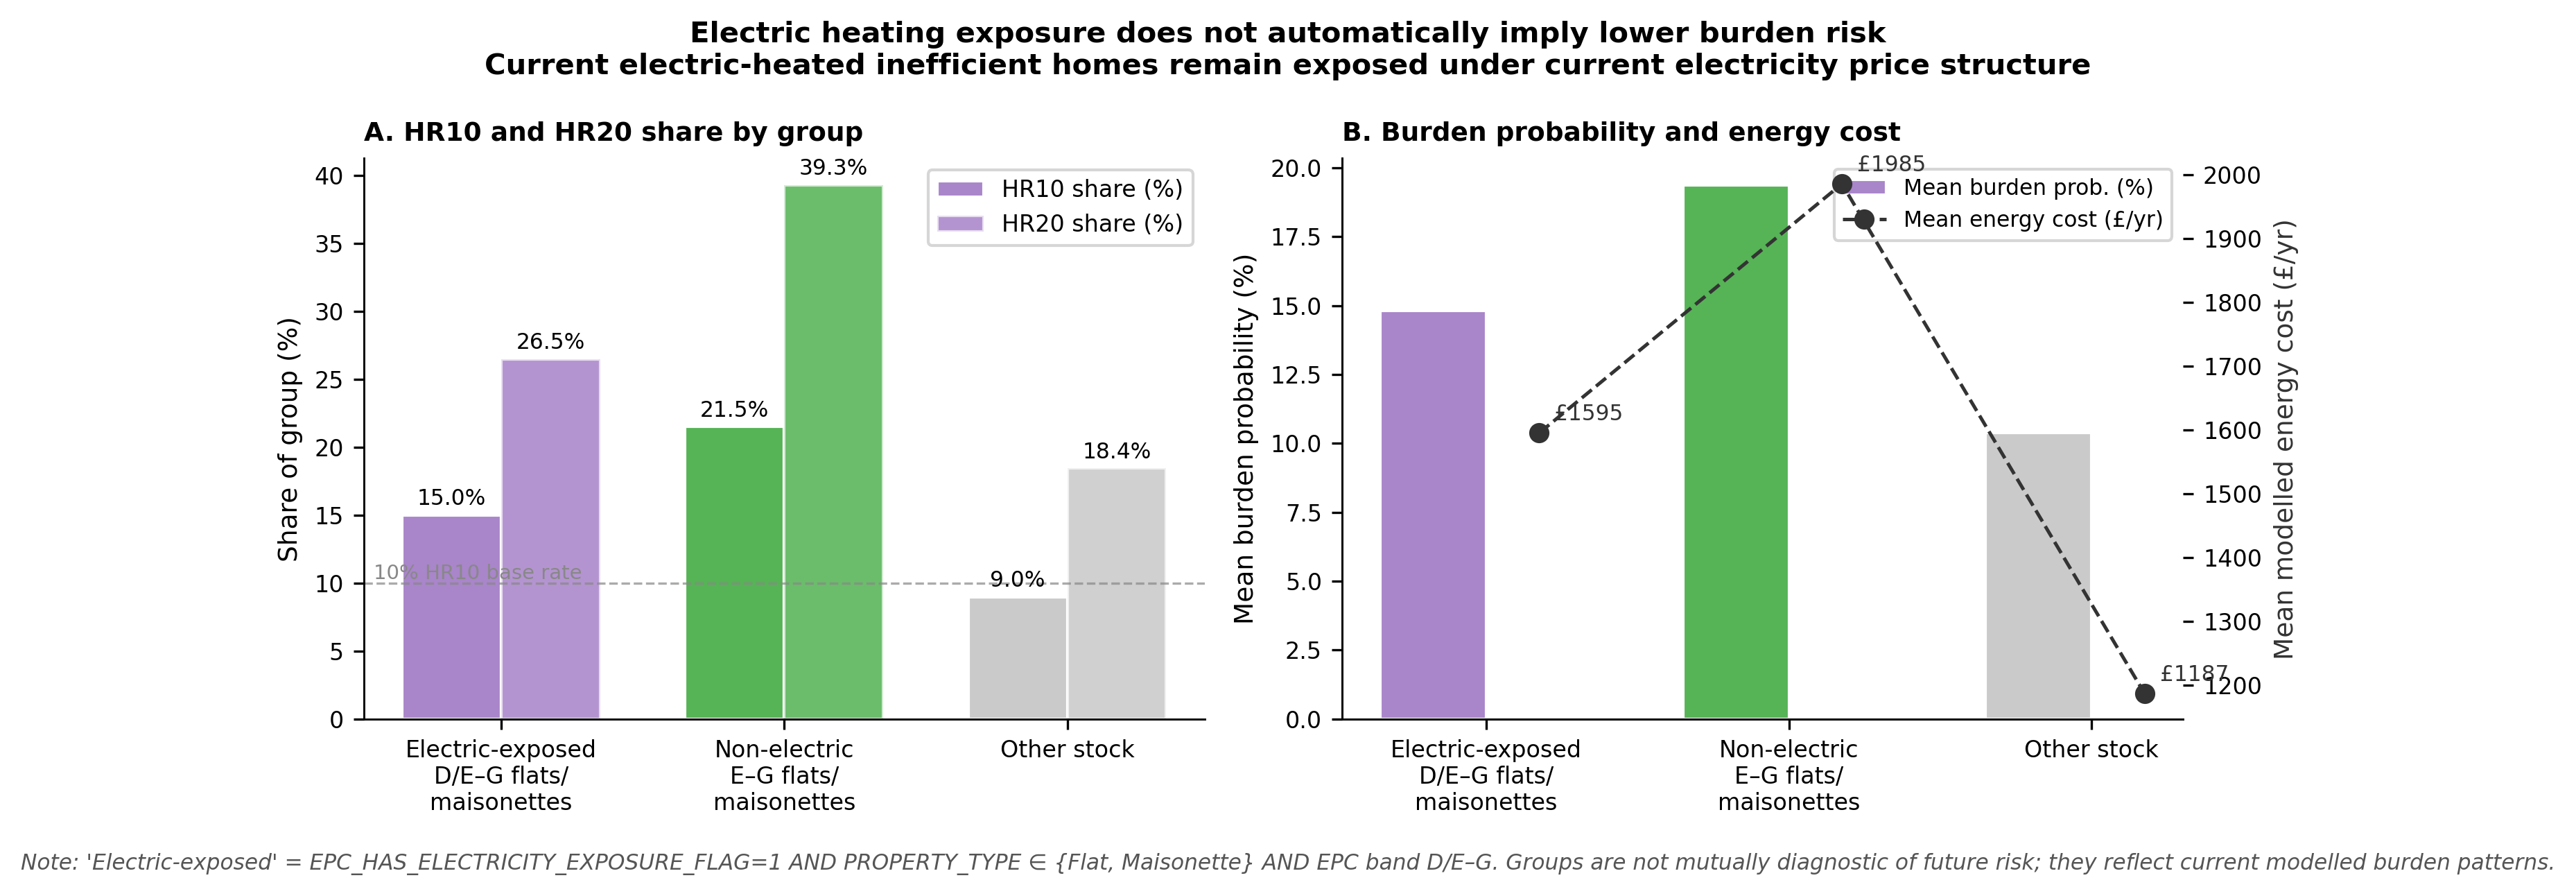
\includegraphics[width=\linewidth]{paper/figures/high_risk_electric_exposure.png}
\caption{Current burden exposure among electric-exposed inefficient flats and maisonettes compared with non-electric low-EPC flats and the rest of the stock. The figure supports the paper's caution that electricity exposure and electrification are not automatically household de-risking mechanisms under current price structures.}
\label{fig:electric-exposure}
\end{figure}

The spatial outputs in Figure~\ref{fig:spatial-high-risk} show that Westminster's current high-burden exposure is geographically uneven and mechanism-specific. They should be interpreted as LSOA-level descriptive maps of current HR10 concentration and dominant HR10 pathway, not as direct maps of future price-shock risk.

\begin{figure}[H]
\centering
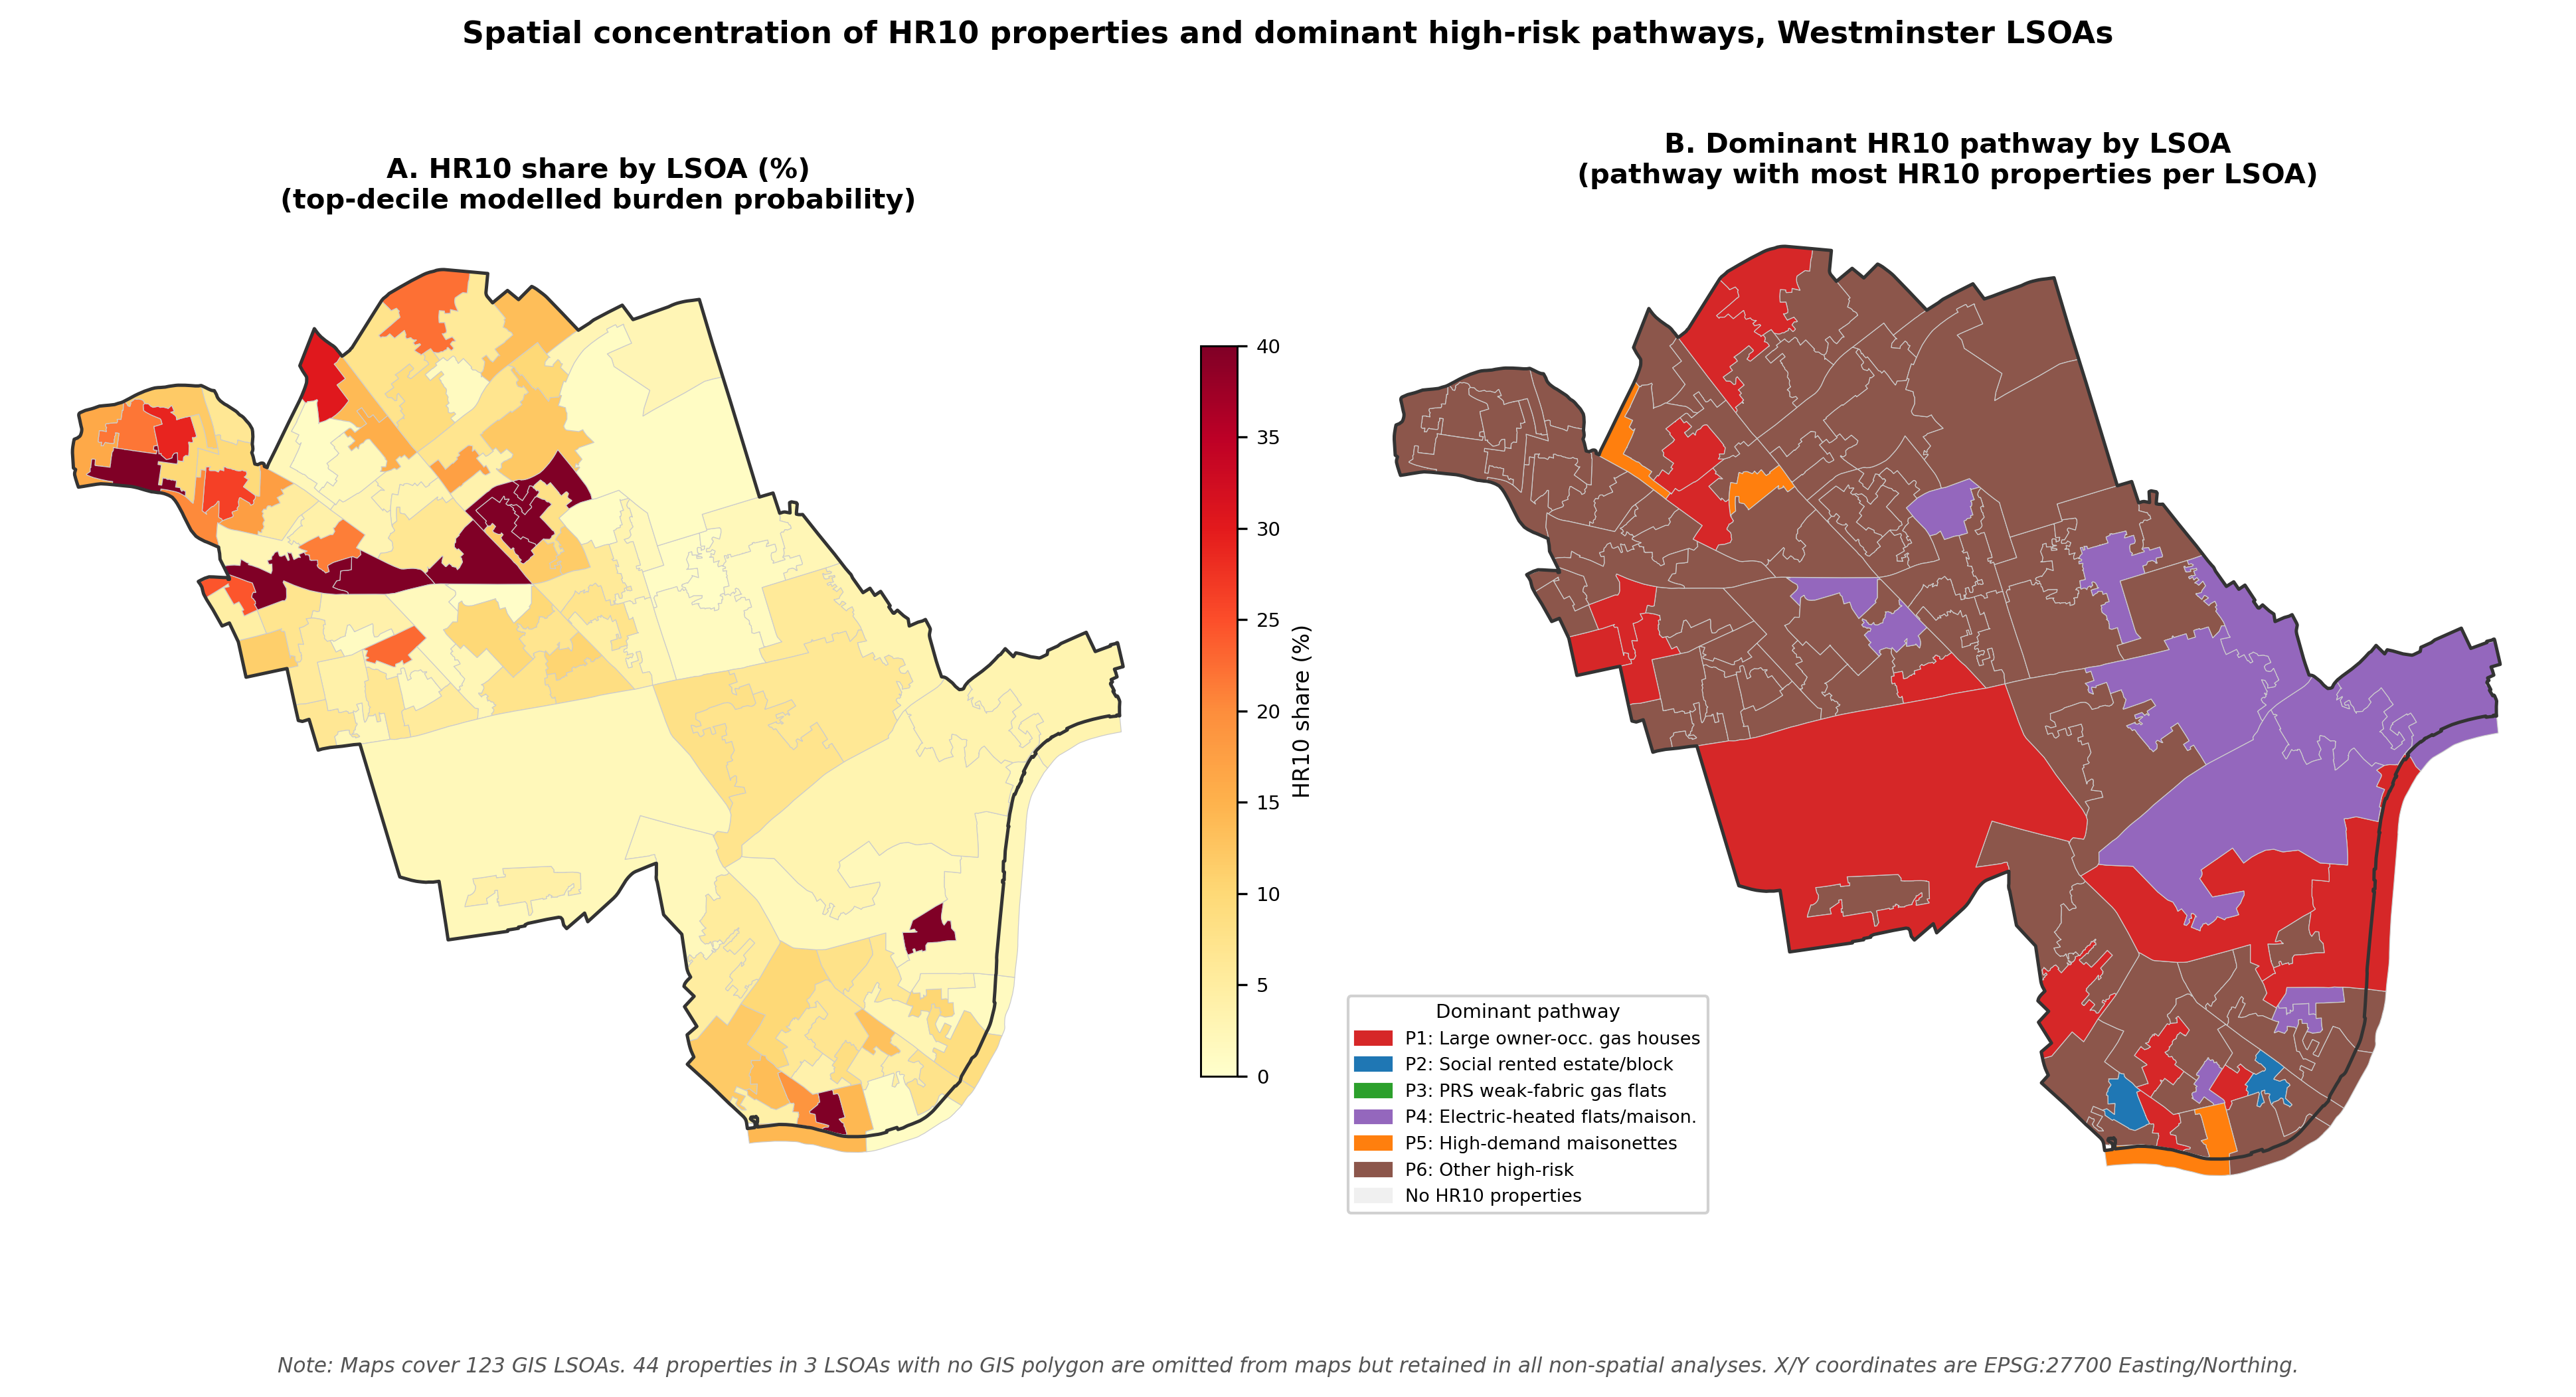
\includegraphics[width=\linewidth]{paper/figures/high_risk_spatial_maps.png}
\caption{Spatial concentration of current modelled HR10 exposure in Westminster. Panel A maps the LSOA share of properties in HR10; Panel B maps the dominant high-risk pathway among HR10 properties in each LSOA. The maps use the 123 LSOAs available in the GIS boundary file.}
\label{fig:spatial-high-risk}
\end{figure}

The residual group is especially important for the next stage. It is too large to remain a black-box category once the paper moves from current exposure into price-shock risk. The planned analysis should separate income-driven residual cases, spatial-deprivation concentrations, mixed housing-and-income mechanisms, and unusual dwelling profiles. This will help distinguish households for whom technical retrofit is the central risk-reduction route from those for whom social tariffs, standing-charge reform, income support, or local assistance may be more relevant.

\subsection{Implemented Official Price-Spine Outputs}

The official price-spine construction adds the price input layer for the next empirical stage. The imported materials report a London monthly domestic spine with 94 S0--S6 rows, an event-level London spine with 22 rows, an all-region Ofgem parser audit, a road-fuel appendix, and a QA summary with no failed checks. These outputs are analytically useful because they allow the paper to model price shocks as specific retail pass-through structures rather than as generic percentage increases. They do not yet estimate household fuel price risk, because required demand, residual income, payment method, fuel connection, and intervention feasibility still need to be joined to the price layer.

Figures~\ref{fig:official-price-spine-timeline}--\ref{fig:official-price-spine-s6} are therefore promoted as method figures. Figure~\ref{fig:official-price-spine-timeline} documents the temporal architecture of S0--S6; Figure~\ref{fig:official-price-spine-unit-rates} shows the unit-rate progression and the S3/S4 policy-buffering contrast; Figure~\ref{fig:official-price-spine-decomposition} keeps unit-rate and standing-charge exposure visible; and Figure~\ref{fig:official-price-spine-s6} identifies the fixed-cost sensitivity that should be interpreted with the documented Q3 proxy caveat. Together, these figures support the scenario engine that will generate burden uplift, threshold crossing, Fuel Price-at-Risk, and de-risking dividends in the next modelling layer.

\subsection{Implemented Price-Shock Result Outputs}

The first price-shock result layer now converts the baseline engine and official price spine into paper-facing evidence on burden uplift and threshold-crossing risk. These outputs use Direct Debit as the central payment-method track and treat Standard Credit and Prepayment as sensitivity tracks until observed household payment-method data are available. The main results focus on S3, S4, and S6 Q3, with S0 and S2 retained as scenario-profile anchors. They should be read as price-shock results, not yet as intervention results: formal Household Fuel Price-at-Risk, affordability gap-at-risk, and de-risking dividend calculations remain the next modelling layer.

Figure~\ref{fig:shock-mechanism-heatmaps} establishes the structural mechanism of exposure under the S3 unmitigated shock. Gas-heated E--G dwellings have a weighted mean required-energy burden uplift of about 10.0 percentage points, compared with about 2.8 percentage points for electricity-heated A--C dwellings. The dwelling-form panel shows a further amplification: E--G houses reach about 12.6 percentage points, while E--G flats are closer to 7.0 percentage points. The result is not simply that inefficient homes are expensive; it is that fuel, fabric, and dwelling form jointly shape price sensitivity.

\begin{figure}[H]
\centering
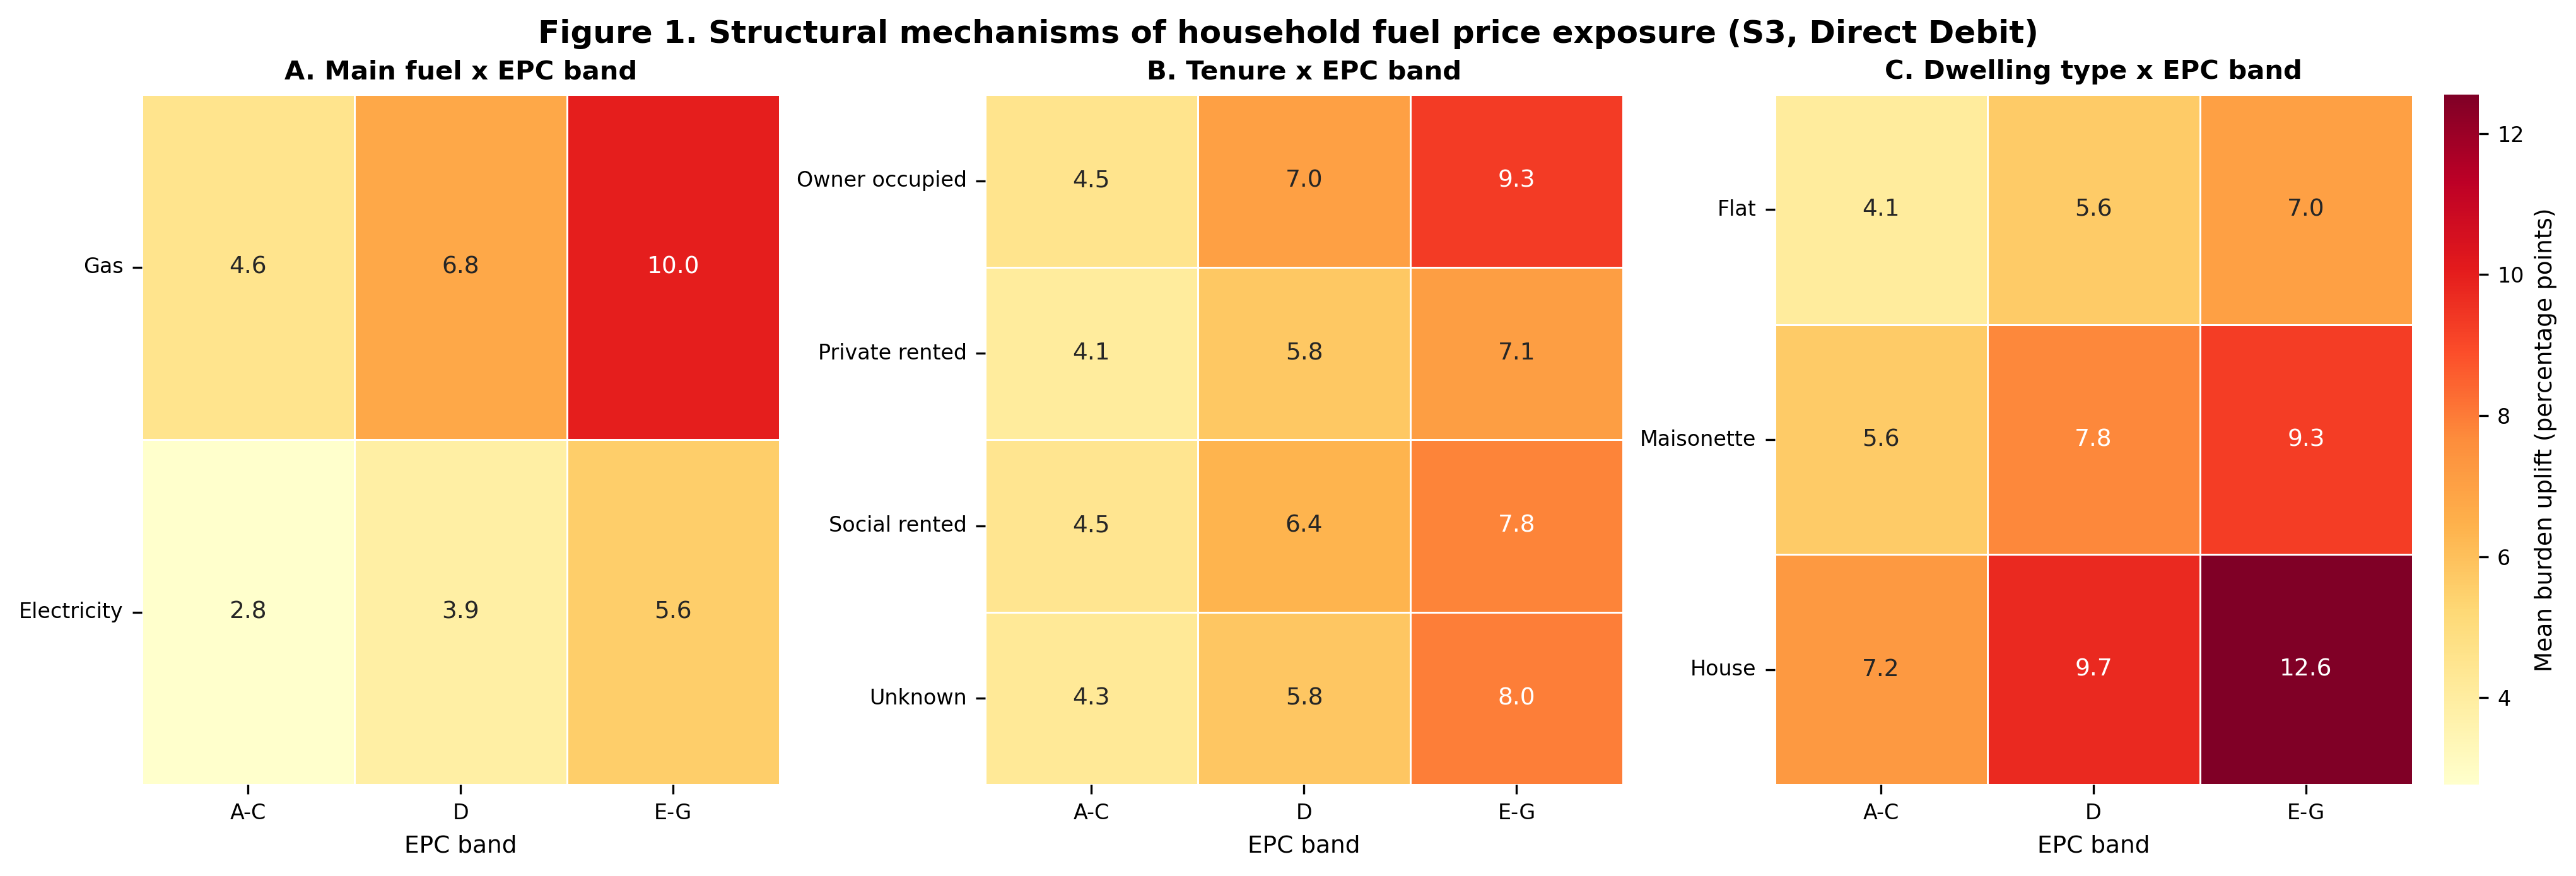
\includegraphics[width=\linewidth]{paper/figures/fuel_price_shock_mechanism_heatmaps.png}
\caption{Weighted mean required-energy burden uplift under the S3 unmitigated price shock, by Westminster dwelling and household-dwelling characteristics. Values are percentage-point changes relative to S0, using Direct Debit as the central payment-method track.}
\label{fig:shock-mechanism-heatmaps}
\end{figure}

Figure~\ref{fig:shock-top-archetypes} then identifies the most exposed household-dwelling archetypes. The highest S3 burden-uplift groups are dominated by gas-heated houses and maisonettes with weak EPC performance. Owner-occupied houses in EPC E--G with gas heating have an average burden uplift of about 13.9 percentage points and a threshold-crossing probability of about 86.7\%; private rented houses in EPC E--G with gas heating follow at about 11.8 percentage points and 81.4\%. The ranking therefore moves the paper beyond generic statements about vulnerable households: exposure is concentrated in specific tenure--dwelling--fabric--fuel combinations.

\begin{figure}[H]
\centering
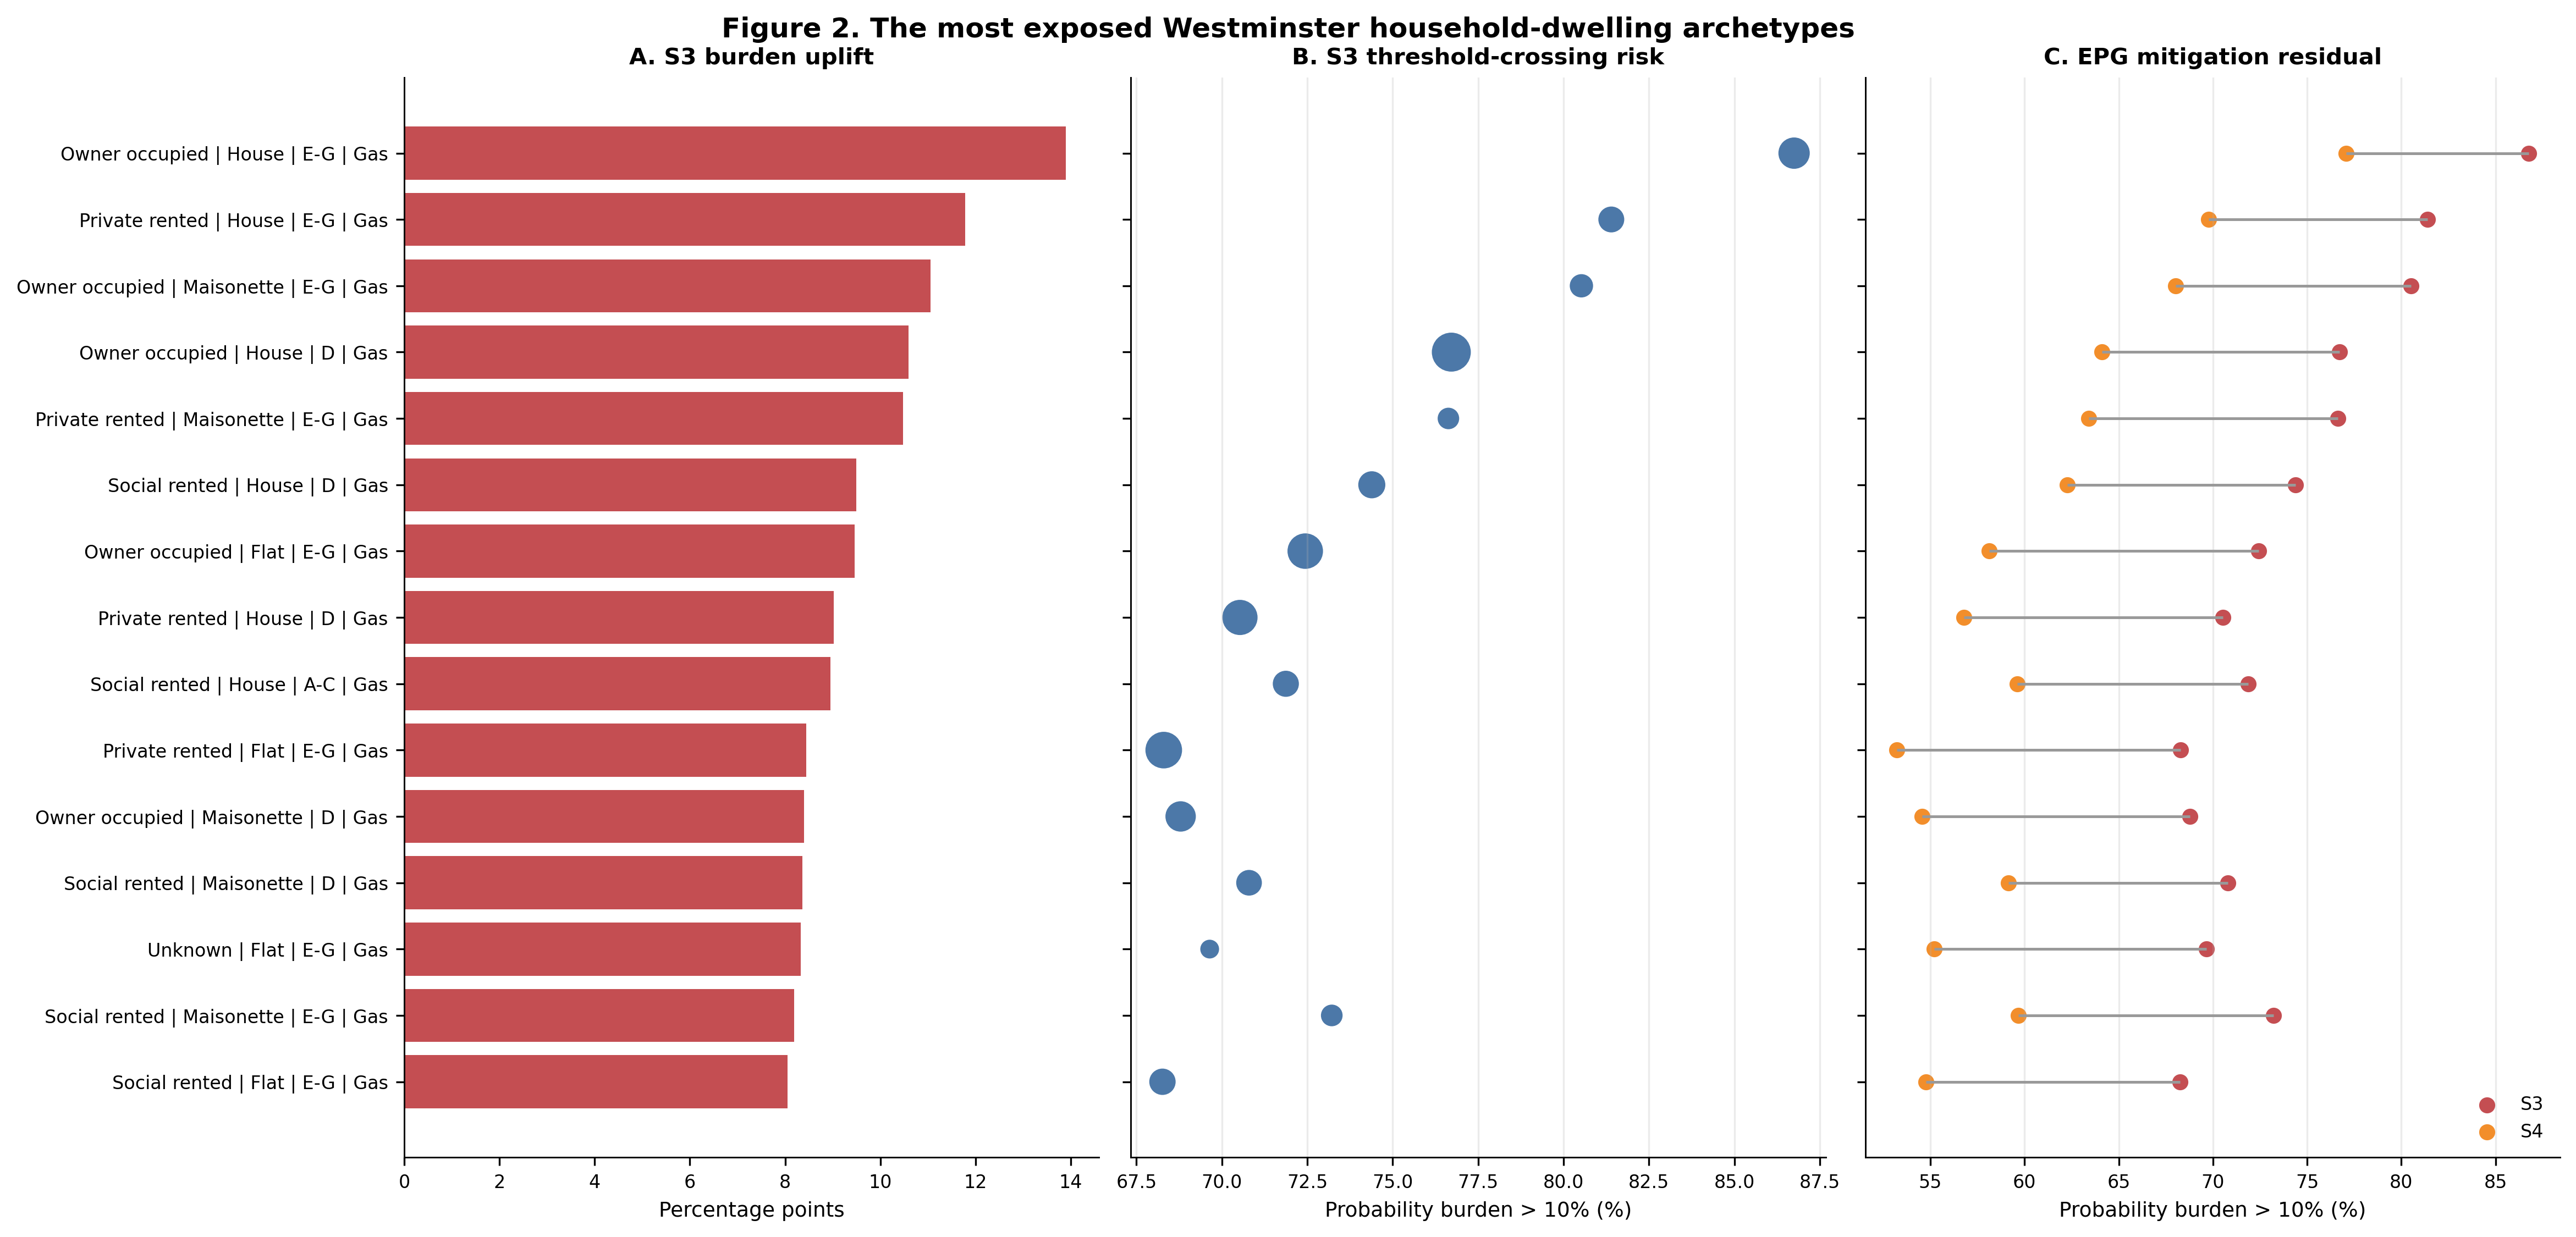
\includegraphics[width=\linewidth]{paper/figures/fuel_price_shock_top_archetype_ranking.png}
\caption{Top Westminster household-dwelling archetypes ranked by S3 required-energy burden uplift, with corresponding S3 threshold-crossing risk and policy-mitigated residual exposure under S4. Archetypes are included where the weighted summary contains at least 100 records.}
\label{fig:shock-top-archetypes}
\end{figure}

Figure~\ref{fig:shock-scenario-profiles} shows how scenario design changes group-level risk. S3 creates a clear risk peak across EPC, fuel, and tenure groups; S4 reduces this exposure through the Energy Price Guarantee; and S6 Q3 leaves a residual fixed-cost and tariff-structure sensitivity. For EPC E--G dwellings, the threshold-crossing probability is about 66.0\% under S3, 51.4\% under S4, and 40.2\% under S6 Q3. The profile supports the paper's distinction between market exposure and policy buffering: mitigation lowers risk but does not remove the underlying inequality in exposure.

\begin{figure}[H]
\centering
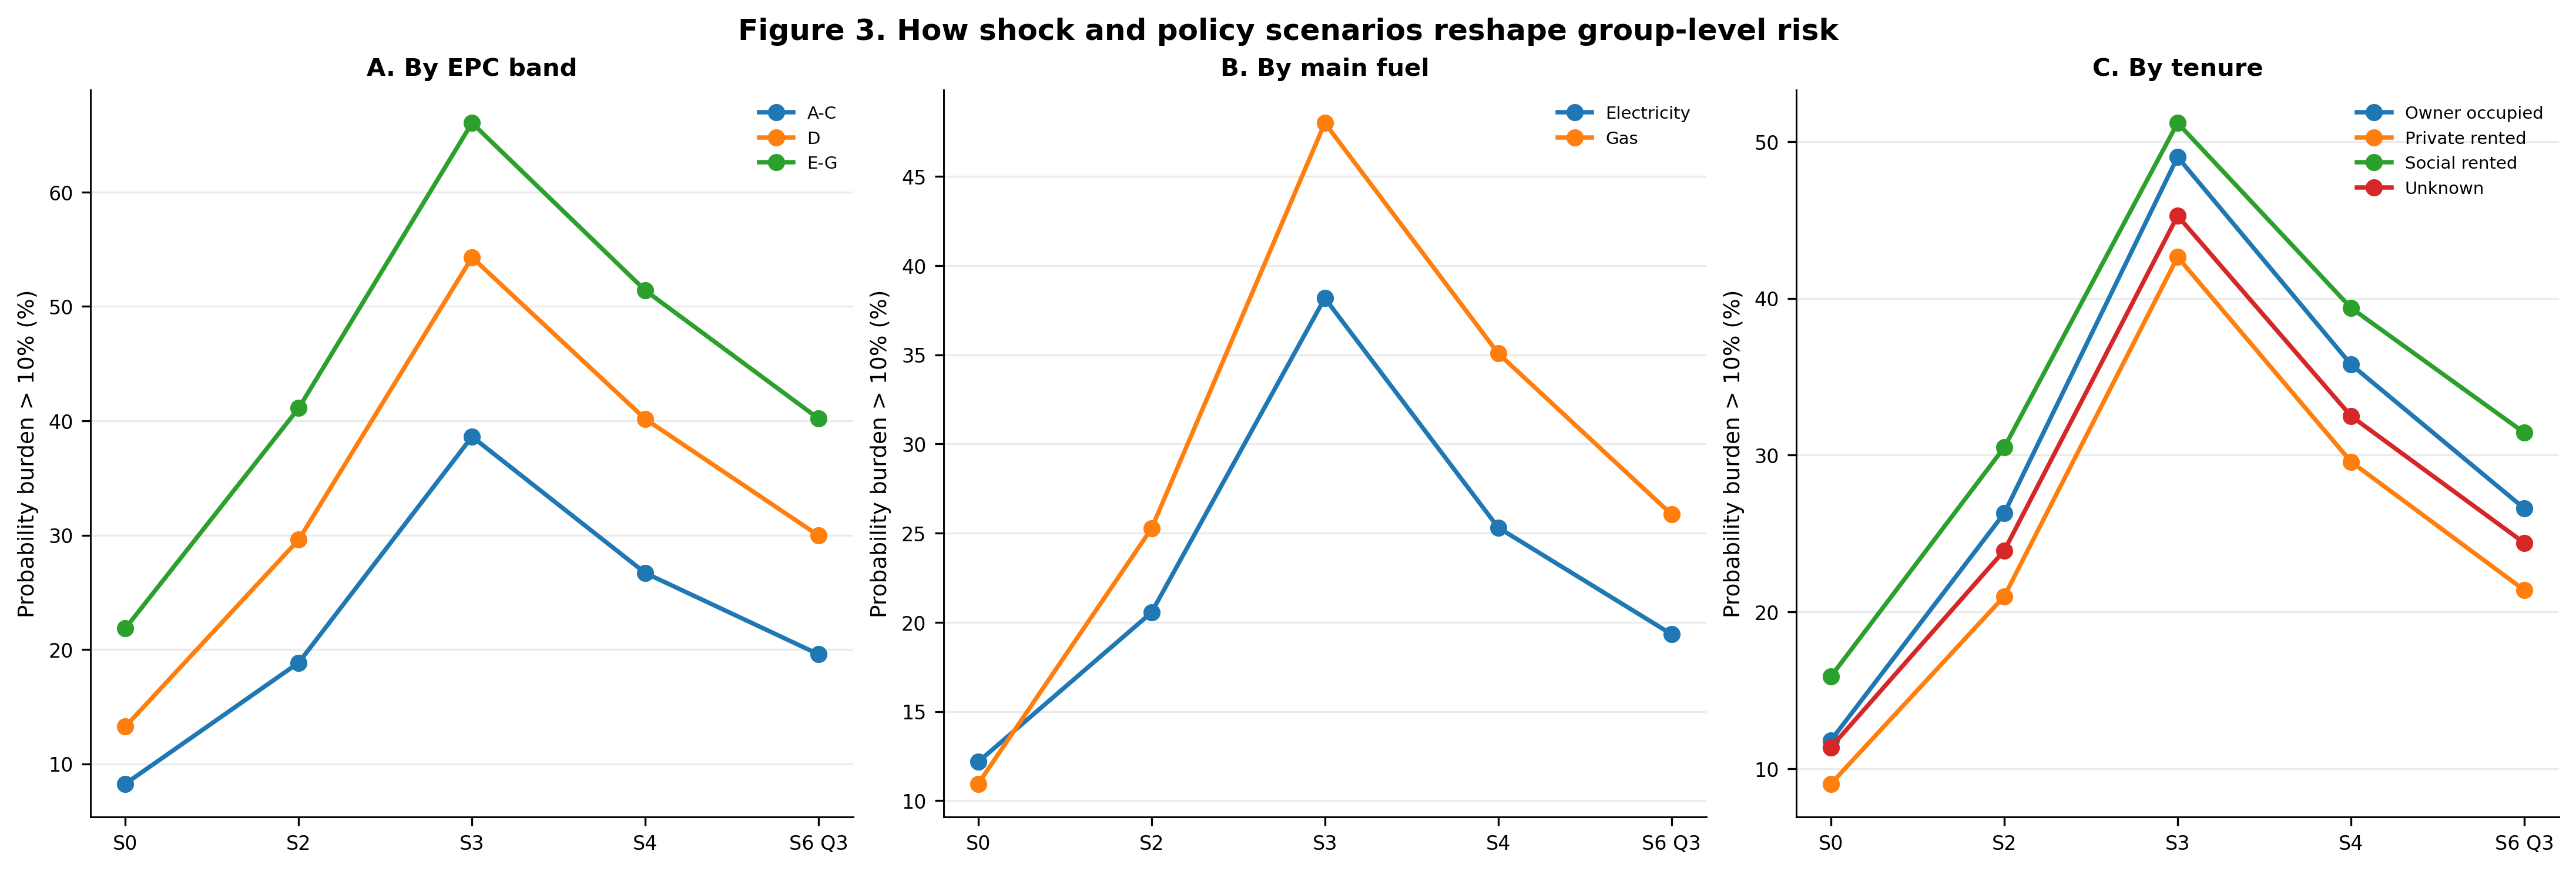
\includegraphics[width=\linewidth]{paper/figures/fuel_price_shock_scenario_response_profiles.png}
\caption{Threshold-crossing probability across S0, S2, S3, S4, and S6 Q3, showing how unmitigated shocks, policy mitigation, and tariff-structure sensitivity reshape group-level household fuel price risk.}
\label{fig:shock-scenario-profiles}
\end{figure}

Finally, Figure~\ref{fig:shock-spatial-distribution} shows that the price-shock burden is spatially concentrated within Westminster. The highest S3 threshold-crossing probabilities in the mapped LSOAs are around 70--76\%, while the diagnostic scatter shows that baseline threshold risk and S3 burden uplift are related but not identical. This spatial result should be interpreted as required-energy price-risk concentration, not as a direct map of observed current fuel poverty. The map uses the 123 LSOAs available in the current GIS boundary file; the three unmatched result LSOAs are retained in non-spatial summaries but omitted from the mapped panels.

\begin{figure}[H]
\centering
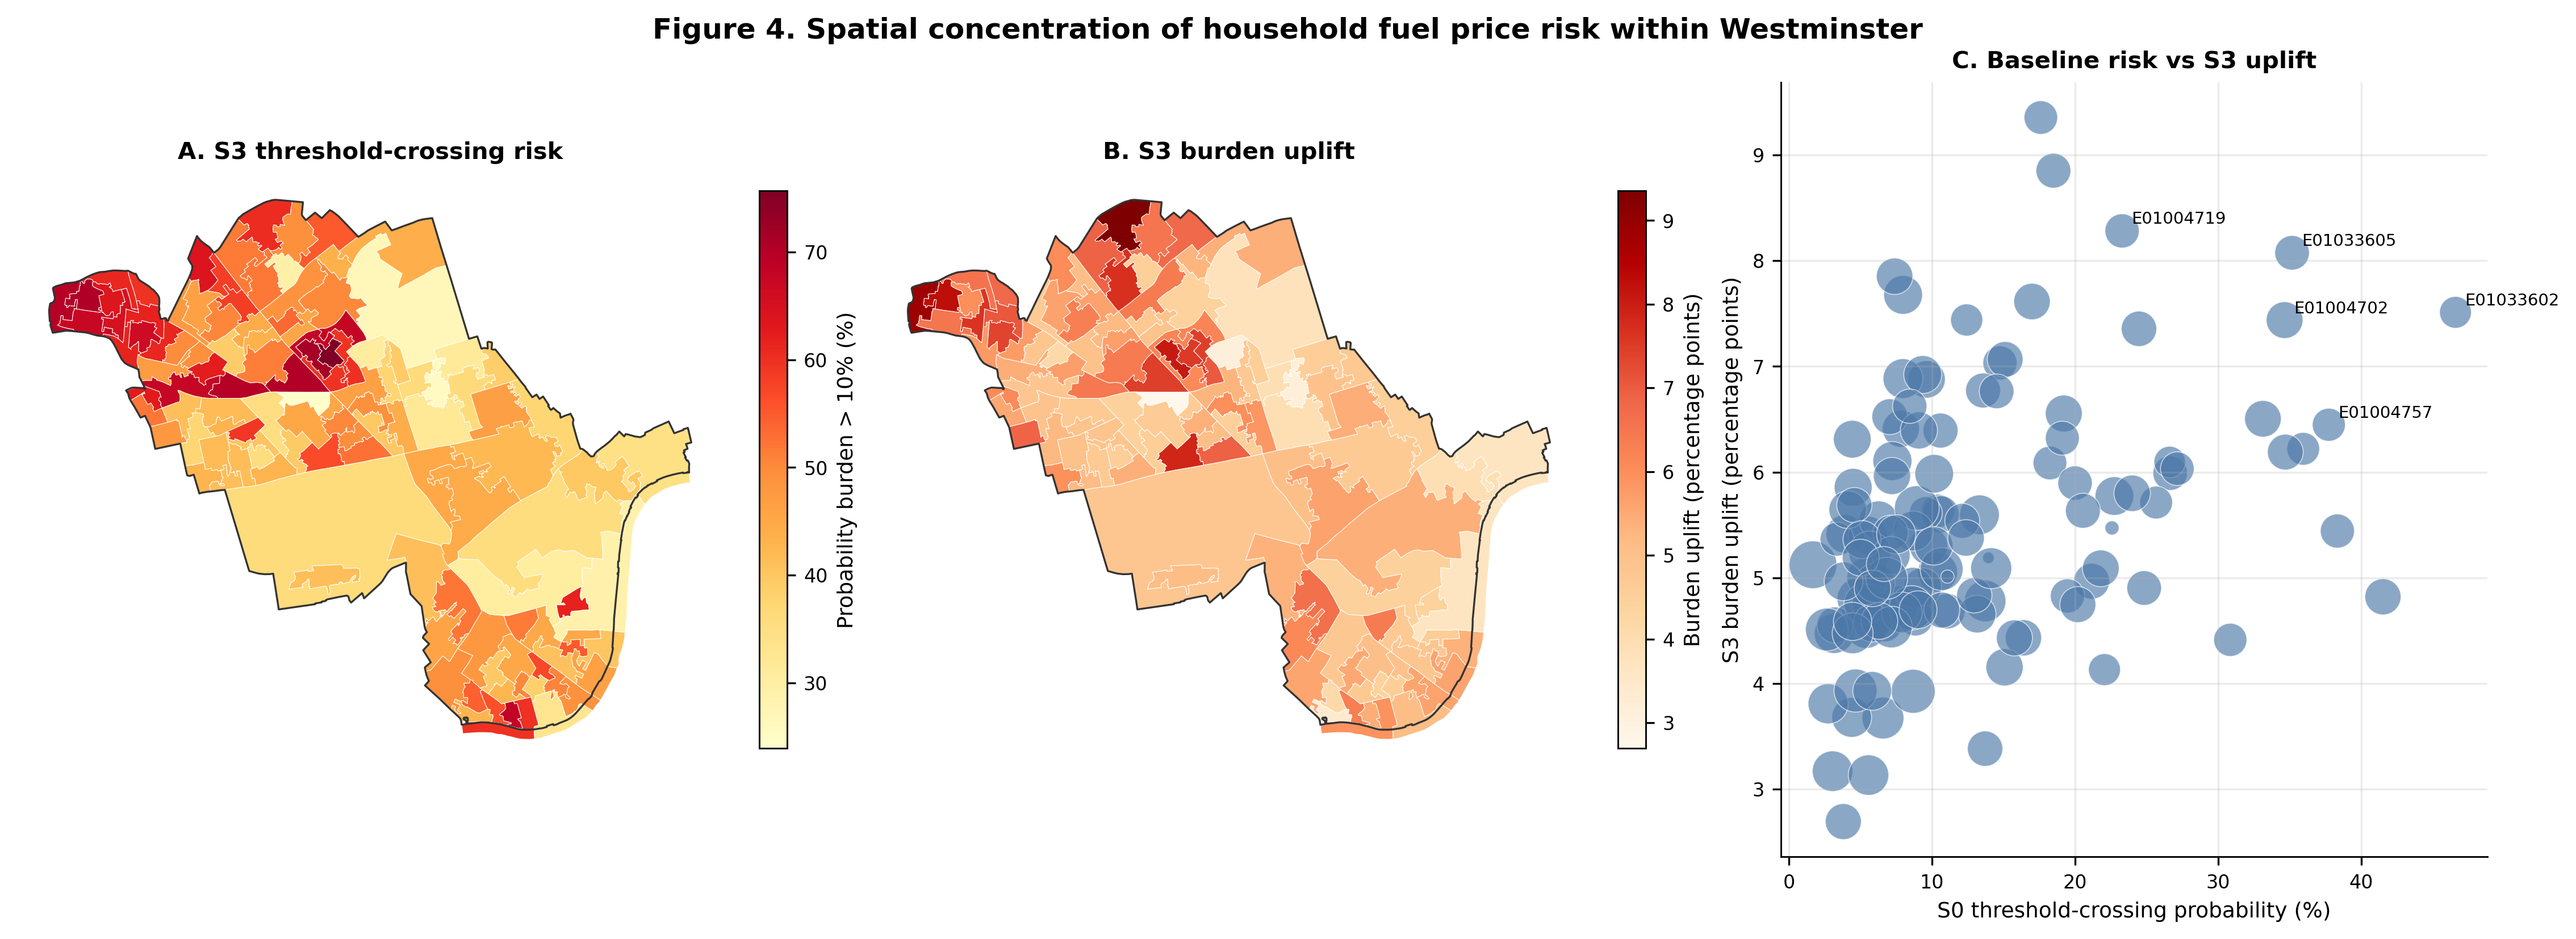
\includegraphics[width=\linewidth]{paper/figures/fuel_price_shock_spatial_distribution.png}
\caption{Spatial concentration of S3 household fuel price risk across Westminster LSOAs. The maps show threshold-crossing probability and required-energy burden uplift; the scatter compares baseline threshold risk with S3 burden uplift.}
\label{fig:shock-spatial-distribution}
\end{figure}

\subsection{Planned Intervention Outputs}

The next empirical layer will estimate intervention-specific protection against the implemented price-shock results. It will compare fabric retrofit, clean heat, PV, battery storage, smart tariffs, and integrated packages under explicit assumptions about technical feasibility, tenure and leasehold governance, roof access, tariff access, electricity/gas price ratios, and policy support. The paper will report not only average burden changes, but also upper-tail risk, burden uplift, threshold-crossing probabilities, and the probability that households remain above policy-relevant burden thresholds after intervention.

The scenario engine should continue to use the baseline extract's applicability fields rather than joining every property to every price scenario. Gas and electricity properties enter S0--S4 and S6 with Direct Debit, Standard Credit, and Prepayment sensitivity labels; oil properties enter only the S5 heating-oil sensitivity. Payment method should remain a scenario dimension unless observed household payment data are added later. This prevents the results from overstating precision or misclassifying oil-heated properties as if they were regulated mains-gas or mains-electricity tariff-cap cases.

A central planned output is the de-risking dividend:
\begin{equation}
\text{De-risking dividend} = \text{Fuel Price-at-Risk}_{\text{before}} - \text{Fuel Price-at-Risk}_{\text{after}}.
\end{equation}
This metric will be estimated by intervention package and household-dwelling condition, including fabric retrofit, clean heat, PV, battery storage, smart tariffs, and integrated packages. Its interpretation will remain conditional: an intervention produces household price-risk protection only where technical feasibility, tenure and leasehold governance, tariff access, electricity/gas price ratios, and market pass-through allow the engineering change to reduce household exposure.

\subsection{Figures and Tables}

Expected tables will summarise baseline burden probabilities, modelled fuel-poverty diagnostics, price-shock burden uplift, Fuel Price-at-Risk, and intervention-specific de-risking dividends by income group, EPC rating, dwelling form, heating system, tenure, payment method, and LSOA/MSOA. The baseline extract figures now promoted into the manuscript are Figures~\ref{fig:baseline-burden-distribution}--\ref{fig:baseline-high-burden-main-fuel}; the current high-risk explanation figures are Figures~\ref{fig:hr-br-overlap}--\ref{fig:spatial-high-risk}; the official price-spine figures are Figures~\ref{fig:official-price-spine-timeline}--\ref{fig:official-price-spine-s6}; and the first price-shock result figures are Figures~\ref{fig:shock-mechanism-heatmaps}--\ref{fig:shock-spatial-distribution}. Remaining expected figures will include: the conceptual distinction between fuel poverty, energy burden, and household fuel price risk; intervention de-risking comparisons; and maps of de-risking gaps.

Before intervention results are reported, the spatial outputs should establish whether different mechanisms concentrate in different parts of Westminster. Priority maps include LSOA HR10 share, LSOA HR20 share, dominant HR10 pathway, social rented estate/block concentration, electric-heated inefficient flat concentration, and residual high-risk concentration. These maps would support the paper's claim that fuel price risk is produced by locally specific combinations of housing form, income sensitivity, and governance constraints rather than by a uniform borough-wide condition.

The synced LSOA income PDF panels from the latest run are included above as Figures~\ref{fig:lsoa-income-pdf-scenarios-1}--\ref{fig:lsoa-income-pdf-scenarios-3}. They show the estimated lognormal income distributions under selected $\lambda$ values, with poverty-line and MSOA-mean markers. They are captioned as synthetic constrained income distributions for burden modelling, not as observed household income distributions and not as direct household fuel price risk outputs.

The paper will ultimately identify de-risking gaps: places and household-dwelling types where fuel price protection is most needed but low-carbon intervention is least accessible. These gaps are expected to be especially important where Westminster's high housing costs, private renting, leasehold flats, heritage constraints, district-heating governance, and uneven tariff or asset access interrupt the translation from domestic net zero investment into household price-risk protection.
